        %%******************************************%%
        %%                                          %%
        %%        Modello di tesi di laurea         %%
        %%            di Andrea Giraldin            %%
        %%                                          %%
        %%             2 novembre 2012              %%
        %%                                          %%
        %%******************************************%%


% I seguenti commenti speciali impostano:
% 1. 
% 2. PDFLaTeX come motore di composizione;
% 3. tesi.tex come documento principale;
% 4. il controllo ortografico italiano per l'editor.

% !TEX encoding = UTF-8
% !TEX TS-program = pdflatex
% !TEX root = tesi.tex
% !TEX spellcheck = it-IT

\documentclass[10pt,                    % corpo del font principale
               a4paper,                 % carta A4
               twoside,                 % impagina per fronte-retro
               openright,               % inizio capitoli a destra
               english,                 
               italian,                 
               ]{book}    

%**************************************************************
% Importazione package
%************************************************************** 

%\usepackage{amsmath,amssymb,amsthm}    % matematica

\usepackage[T1]{fontenc}                % codifica dei font:
                                        % NOTA BENE! richiede una distribuzione *completa* di LaTeX

\usepackage{libertine}
\usepackage{libertinust1math}
\usepackage{lmodern}

\usepackage[utf8]{inputenc}             % codifica di input; anche [latin1] va bene
                                        % NOTA BENE! va accordata con le preferenze dell'editor

\usepackage[english, italian]{babel}    % per scrivere in italiano e in inglese;
                                        % l'ultima lingua (l'italiano) risulta predefinita

\usepackage{bookmark}                   % segnalibri

\usepackage{caption}                    % didascalie

\usepackage{chngpage,calc}              % centra il frontespizio

\usepackage{csquotes}                   % gestisce automaticamente i caratteri (")

\usepackage{emptypage}                  % pagine vuote senza testatina e piede di pagina

\usepackage{epigraph}			% per epigrafi

\usepackage{eurosym}                    % simbolo dell'euro

%\usepackage{indentfirst}               % rientra il primo paragrafo di ogni sezione

\usepackage{graphicx}                   % immagini

\usepackage{hyperref}                   % collegamenti ipertestuali

\usepackage[binding=5mm]{layaureo}      % margini ottimizzati per l'A4; rilegatura di 5 mm

\usepackage{listings}                   % codici

\usepackage{microtype}                  % microtipografia

\usepackage{mparhack,fixltx2e,relsize}  % finezze tipografiche

\usepackage{nameref}                    % visualizza nome dei riferimenti                                      

\usepackage[font=small]{quoting}        % citazioni

\usepackage{subfig}                     % sottofigure, sottotabelle

\usepackage[italian]{varioref}          % riferimenti completi della pagina

\usepackage[dvipsnames]{xcolor}         % colori

\usepackage{booktabs}                   % tabelle                                       
\usepackage{tabularx}                   % tabelle di larghezza prefissata                                    
\usepackage{longtable}                  % tabelle su più pagine                                        
\usepackage{ltxtable}                   % tabelle su più pagine e adattabili in larghezza

\usepackage[toc, acronym]{glossaries}   % glossario
                                        % per includerlo nel documento bisogna:
                                        % 1. compilare una prima volta tesi.tex;
                                        % 2. eseguire: makeindex -s tesi.ist -t tesi.glg -o tesi.gls tesi.glo
                                        % 3. eseguire: makeindex -s tesi.ist -t tesi.alg -o tesi.acr tesi.acn
                                        % 4. compilare due volte tesi.tex.

\usepackage[backend=biber,style=verbose-ibid,hyperref,backref]{biblatex}
                                        % eccellente pacchetto per la bibliografia; 
                                        % produce uno stile di citazione autore-anno; 
                                        % lo stile "numeric-comp" produce riferimenti numerici
                                        % per includerlo nel documento bisogna:
                                        % 1. compilare una prima volta tesi.tex;
                                        % 2. eseguire: biber tesi
                                        % 3. compilare ancora tesi.tex.

%**************************************************************
% file contenente le impostazioni della tesi
%**************************************************************

%**************************************************************
% Frontespizio
%**************************************************************


% Autore
\newcommand{\myName}{Riccardo Basso}                                    
\newcommand{\myTitle}{Sviluppo di algoritmi euristici di ottimizzazione e applicazione alla pianificazione della produzione}

% Tipo di tesi                   
\newcommand{\myDegree}{Tesi di laurea triennale}

% Università             
\newcommand{\myUni}{Università degli Studi di Padova}

% Facoltà       
\newcommand{\myFaculty}{Corso di Laurea in Informatica}

% Dipartimento
\newcommand{\myDepartment}{Dipartimento di Matematica "Tullio Levi-Civita"}

% Titolo del relatore
\newcommand{\profTitle}{Prof. }

% Relatore
\newcommand{\myProf}{Luigi De Giovanni}

% Luogo
\newcommand{\myLocation}{Padova}

% Anno accademico
\newcommand{\myAA}{2018-2019}

% Data discussione
\newcommand{\myTime}{Dicembre 2019}


%**************************************************************
% Impostazioni di impaginazione
% see: http://wwwcdf.pd.infn.it/AppuntiLinux/a2547.htm
%**************************************************************

\setlength{\parindent}{14pt}   % larghezza rientro della prima riga
\setlength{\parskip}{0pt}   % distanza tra i paragrafi


%**************************************************************
% Impostazioni di biblatex
%**************************************************************
\bibliography{bibliografia} % database di biblatex 

\defbibheading{bibliography} {
    %\cleardoublepage
    \phantomsection 
    \addcontentsline{toc}{chapter}{\bibname}
    \chapter*{\bibname\markboth{\bibname}{\bibname}}
}

\setlength\bibitemsep{1.5\itemsep} % spazio tra entry

\DeclareBibliographyCategory{opere}
\DeclareBibliographyCategory{web}

\addtocategory{opere}{womak:lean-thinking}
\addtocategory{web}{site:agile-manifesto}

\defbibheading{opere}{\section*{Riferimenti bibliografici}}
\defbibheading{web}{\section*{Siti Web consultati}}


%**************************************************************
% Impostazioni di caption
%**************************************************************
\captionsetup{
    tableposition=bottom,
    figureposition=bottom,
    font=small,
    format=hang,
    labelfont=bf
}

%**************************************************************
% Impostazioni di glossaries
%**************************************************************
\newcommand{\glo}{$_{G}$}
\newcommand{\glosp}{$_{G}$ }

%**************************************************************
% Impostazioni di graphicx
%**************************************************************
\graphicspath{{immagini/}} % cartella dove sono riposte le immagini


%**************************************************************
% Impostazioni di hyperref
%**************************************************************
\hypersetup{
    %hyperfootnotes=false,
    %pdfpagelabels,
    %draft,	% = elimina tutti i link (utile per stampe in bianco e nero)
    colorlinks=false,
    linktoc=all,
    pdfstartpage=1,
    pdfstartview=FitV,
    % decommenta la riga seguente per avere link in nero (per esempio per la stampa in bianco e nero)
    %colorlinks=false, linktocpage=false, pdfborder={0 0 0}, pdfstartpage=1, pdfstartview=FitV,
    breaklinks=true,
    pdfpagemode=UseNone,
    pageanchor=true,
    pdfpagemode=UseOutlines,
    plainpages=false,
    bookmarksnumbered,
    bookmarksopen=true,
    bookmarksopenlevel=1,
    hypertexnames=true,
    pdfhighlight=/O,
    %nesting=true,
    %frenchlinks,
    urlcolor=webbrown,
    linkcolor=RoyalBlue,
    citecolor=webgreen,
    %pagecolor=RoyalBlue,
    %urlcolor=Black, linkcolor=Black, citecolor=Black, %pagecolor=Black,
    pdftitle={\myTitle},
    pdfauthor={\textcopyright\ \myName, \myUni, \myFaculty},
    pdfsubject={},
    pdfkeywords={},
    pdfcreator={pdfLaTeX},
    pdfproducer={LaTeX}
}

%**************************************************************
% Impostazioni di listings
%**************************************************************
\lstset{
    language=[LaTeX]Tex,%C++,
    keywordstyle=\color{RoyalBlue}, %\bfseries,
    basicstyle=\small\ttfamily,
    %identifierstyle=\color{NavyBlue},
    commentstyle=\color{Green}\ttfamily,
    stringstyle=\rmfamily,
    numbers=none, %left,%
    numberstyle=\scriptsize, %\tiny
    stepnumber=5,
    numbersep=8pt,
    showstringspaces=false,
    breaklines=true,
    frameround=ftff,
    frame=single
} 


%**************************************************************
% Impostazioni di xcolor
%**************************************************************
%\definecolor{webgreen}{rgb}{0,.5,0}
%\definecolor{webbrown}{rgb}{.6,0,0}


%**************************************************************
% Altro
%**************************************************************

\newcommand{\omissis}{[\dots\negthinspace]} % produce [...]

% eccezioni all'algoritmo di sillabazione
\hyphenation
{
    ma-cro-istru-zio-ne
    gi-ral-din
}

\newcommand{\sectionname}{sezione}
\addto\captionsitalian{\renewcommand{\figurename}{Figura}
                       \renewcommand{\tablename}{Tabella}}

\newcommand{\glsfirstoccur}{\ap{{[g]}}}

\newcommand{\intro}[1]{\emph{\textsf{#1}}}

%**************************************************************
% Environment per ``rischi''
%**************************************************************
\newcounter{riskcounter}                % define a counter
\setcounter{riskcounter}{0}             % set the counter to some initial value

%%%% Parameters
% #1: Title
\newenvironment{risk}[1]{
    \refstepcounter{riskcounter}        % increment counter
    \par \noindent                      % start new paragraph
    \textbf{\arabic{riskcounter}. #1}   % display the title before the 
                                        % content of the environment is displayed 
}{
    \par\medskip
}

\newcommand{\riskname}{Rischio}

\newcommand{\riskdescription}[1]{\textbf{\\Descrizione:} #1.}

\newcommand{\risksolution}[1]{\textbf{\\Soluzione:} #1.}

%**************************************************************
% Environment per ``use case''
%**************************************************************
\newcounter{usecasecounter}             % define a counter
\setcounter{usecasecounter}{0}          % set the counter to some initial value

%%%% Parameters
% #1: ID
% #2: Nome
\newenvironment{usecase}[2]{
    \renewcommand{\theusecasecounter}{\usecasename #1}  % this is where the display of 
                                                        % the counter is overwritten/modified
    \refstepcounter{usecasecounter}             % increment counter
    \vspace{10pt}
    \par \noindent                              % start new paragraph
    {\large \textbf{\usecasename #1: #2}}       % display the title before the 
                                                % content of the environment is displayed 
    \medskip
}{
    \medskip
}

\newcommand{\usecasename}{UC}

\newcommand{\usecaseactors}[1]{\textbf{\\Attori Principali:} #1. \vspace{4pt}}
\newcommand{\usecasepre}[1]{\textbf{\\Precondizioni:} #1. \vspace{4pt}}
\newcommand{\usecasedesc}[1]{\textbf{\\Descrizione:} #1. \vspace{4pt}}
\newcommand{\usecasepost}[1]{\textbf{\\Postcondizioni:} #1. \vspace{4pt}}
\newcommand{\usecasealt}[1]{\textbf{\\Scenario Alternativo:} #1. \vspace{4pt}}

%***************************************************
%Comandi tabelle
%***************************************************
% multirow per tabelle
\usepackage{multirow}

% Permette tabelle su più pagine

\usepackage{longtable}


% colore di sfondo per le celle
%\usepackage{xcolor}

%COMANDI TABELLE
\newcommand{\rowcolorhead}{\rowcolor[HTML]{56A5EC}} %intestazione 
\newcommand{\rowcolorlight}{\rowcolor[HTML]{FAFAFA}} %righe chiare/dispari
\newcommand{\rowcolordark}{\rowcolor[HTML]{E1F5FE}} %righe scure/pari
\newcommand{\colorhead}{\color[HTML]{FFFFFF}} %testo intestazione
\newcommand{\colorbody}{\color[HTML]{000000}} %testo righe
\newcommand{\tabitem}{~~\rlap{\textbullet}~~}

\definecolor{pari}{HTML}{E1F5FE}
\definecolor{dispari}{HTML}{FAFAFA}


%**************************************************************
% Environment per ``namespace description''
%**************************************************************

\newenvironment{namespacedesc}{
    \vspace{10pt}
    \par \noindent                              % start new paragraph
    \begin{description} 
}{
    \end{description}
    \medskip
}

\newcommand{\classdesc}[2]{\item[\textbf{#1:}] #2}                     % file con le impostazioni personali

\begin{document}
%**************************************************************
% Materiale iniziale
%**************************************************************
\frontmatter
% !TEX encoding = UTF-8
% !TEX TS-program = pdflatex
% !TEX root = ../tesi.tex

%**************************************************************
% Frontespizio 
%**************************************************************
\begin{titlepage}

\begin{center}

\begin{LARGE}
\textbf{\myUni}\\
\end{LARGE}

\vspace{10pt}

\begin{Large}
\textsc{\myDepartment}\\
\end{Large}

\vspace{10pt}

\begin{large}
\textsc{\myFaculty}\\
\end{large}

\vspace{30pt}
\begin{figure}[htbp]
\begin{center}

\includegraphics[height=6cm]{logo-unipd}
\end{center}
\end{figure}
\vspace{30pt} 

\begin{LARGE}
\begin{center}
\textbf{\myTitle}\\
\end{center}
\end{LARGE}

\vspace{10pt} 

\begin{large}
\textsl{\myDegree}\\
\end{large}

\vspace{40pt} 

\begin{large}
\begin{flushleft}
\textit{Relatore}\\ 
\vspace{5pt} 
\profTitle \myProf
\end{flushleft}

\vspace{0pt} 

\begin{flushright}
\textit{Laureando}\\ 
\vspace{5pt} 
\myName
\end{flushright}
\end{large}

\vspace{40pt}

\line(1, 0){338} \\
\begin{normalsize}
\textsc{Anno Accademico \myAA}
\end{normalsize}

\end{center}
\end{titlepage} 
% !TEX encoding = UTF-8
% !TEX TS-program = pdflatex
% !TEX root = ../tesi.tex

%**************************************************************
% Colophon
%**************************************************************
\clearpage
\phantomsection
\thispagestyle{empty}

\hfill

\vfill

\noindent\myName: \textit{\myTitle,}
\myDegree,
\textcopyright\ \myTime.
% !TEX encoding = UTF-8
% !TEX TS-program = pdflatex
% !TEX root = ../tesi.tex

%**************************************************************
% Dedica
%**************************************************************
\cleardoublepage
\phantomsection
\thispagestyle{empty}


% !TEX encoding = UTF-8
% !TEX TS-program = pdflatex
% !TEX root = ../tesi.tex

%**************************************************************
% Sommario
%**************************************************************
\cleardoublepage
\phantomsection
\pdfbookmark{Sommario}{Sommario}
\begingroup
\let\clearpage\relax
\let\cleardoublepage\relax
\let\cleardoublepage\relax

\chapter*{Sommario}

Il presente documento descrive il lavoro svolto durante il periodo di stage, della durata di circa trecentoventi ore, dal laureando Basso Riccardo presso l'azienda Ergon Informatica. 
Gli obbiettivi da raggiungere erano molteplici e sono descritti nei seguenti capitoli.\\
Il primo capitolo tratta dell'azienda e del suo rapporto con l'università.\\
Il secondo capitolo fornisce un'idea generale del progetto di stage, accompagnata dall'analisi dei rischi.\\
Il terzo capitolo racchiude il tracciamento dei requisiti e descrive le varie tecnologie utilizzate durante il progetto.\\
Il quarto capitolo parla in dettaglio del progetto di stage e di come è stato svolto. Racchiude una panoramica iniziale dell'architettura per poi soffermarsi in dettaglio
sull'analisi del problema stesso e della sua soluzione. Si conclude con i risultati dei test effettuati.\\
Il quinto e ultimo capitolo racchiude le varie conclusioni raggiunte al termine dello stage.\\


%\vfill
%
%\selectlanguage{english}
%\pdfbookmark{Abstract}{Abstract}
%\chapter*{Abstract}
%
%\selectlanguage{italian}

\endgroup			

\vfill


% !TEX encoding = UTF-8
% !TEX TS-program = pdflatex
% !TEX root = ../tesi.tex

%**************************************************************
% Ringraziamenti
%**************************************************************
\cleardoublepage
\phantomsection
\pdfbookmark{Ringraziamenti}{ringraziamenti}

\begin{flushright}{
	\slshape    
	``Life is really simple, but we insist on making it complicated''} \\ 
	\medskip
    --- Confucius
\end{flushright}


\bigskip

\begingroup
\let\clearpage\relax
\let\cleardoublepage\relax
\let\cleardoublepage\relax

\chapter*{Ringraziamenti}

\noindent \textit{Innanzitutto, vorrei esprimere la mia gratitudine al Prof. NomeDelProfessore, relatore della mia tesi, per l'aiuto e il sostegno fornitomi durante la stesura del lavoro.}\\

\noindent \textit{Desidero ringraziare con affetto i miei genitori per il sostegno, il grande aiuto e per essermi stati vicini in ogni momento durante gli anni di studio.}\\

\noindent \textit{Ho desiderio di ringraziare poi i miei amici per tutti i bellissimi anni passati insieme e le mille avventure vissute.}\\
\bigskip

\noindent\textit{\myLocation, \myTime}
\hfill \myName

\endgroup


% !TEX encoding = UTF-8
% !TEX TS-program = pdflatex
% !TEX root = ../tesi.tex

%**************************************************************
% Indici
%**************************************************************
\cleardoublepage
\pdfbookmark{\contentsname}{tableofcontents}
\setcounter{tocdepth}{2}
\tableofcontents
%\markboth{\contentsname}{\contentsname} 
\clearpage

\begingroup 
    \let\clearpage\relax
    \let\cleardoublepage\relax
    \let\cleardoublepage\relax
    %*******************************************************
    % Elenco delle figure
    %*******************************************************    
    \phantomsection
    \pdfbookmark{\listfigurename}{lof}
    \listoffigures

    \vspace*{8ex}

    %*******************************************************
    % Elenco delle tabelle
    %*******************************************************
    \phantomsection
    \pdfbookmark{\listtablename}{lot}
    \listoftables
        
    \vspace*{8ex}
\endgroup

\cleardoublepage

\cleardoublepage

%**************************************************************
% Materiale principale
%**************************************************************
\mainmatter
% !TEX encoding = UTF-8
% !TEX TS-program = pdflatex
% !TEX root = ../tesi.tex

%**************************************************************
\chapter{Introduzione}
\label{cap:introduzione}

\section{L'azienda}

Ergon Informatica\hyperref[sec:ergon]{[1]} viene fondata nel 1988 come società di Ingegneria Informatica per applicazioni gestionali dedicate.
La società, che all'inizio conta solo alcuni dipendenti, si sviluppa in maniera costante negli anni e oggi può vantare una posizione di tutto rispetto tra le aziende dello stesso settore.
I clienti iniziali hanno giocato un ruolo fondamentale nello sviluppo del software prodotto da Ergon; essi infatti appartenevano per la maggior parte all'ambito alimentare e l'esperienza di queste prime installazioni ha permesso di acquisire delle competenze interne altamente specializzate in questo settore.
\subsection{Organizzazione aziendale}
Attualmente fanno parte della stessa gestione tre società:

\begin{itemize}
\item Ergon Informatica S.r.l. che si occupa dello sviluppo software, in particolare del gestionale Ergdis;
\item Ergon S.r.l. che si occupa dei servizi tecnologici;
\item Ergon Servizi S.r.l. che si occupa dei servizi amministrativi, logistici e di marketing delle sopracitate.
\end{itemize}
\newpage
\subsection{Servizi aziendali}
Vengono di seguito presentati l'insieme dei servizi proposti dall'azienda Ergon Informatica:
\begin{itemize}
	\item \textbf{Help Desk}: Il servizio di assistenza è fornito tramite un'apertura di chiamata che può essere effettuata via web o telefonando presso la sede.
	Un servizio di monitoring  interno permette di individuare gli eventuali ritardi nelle risposte e negli interventi risolutivi. Il sistema di qualità ( ISO 9001), che Ergon ha adottato, individua un tempo massimo di risoluzione del problema.
	Il cliente, collegandosi all'area a lui riservata, ha la possibilità di monitorare tutte le sue chiamate e verificare, per quelle ancora aperte,
	 il tempo  previsto di chiusura;
	\item \textbf{Servizio di Monitoring}: Il servizio prevede l'installazione per ogni server di un certo numero di agenti.
	Un operatore di Ergon, da remoto, attraverso un programma di controllo, rileva i vari tipi di \hyperref[Alert]{"alert"\glosp}  e, in accordo con il cliente, 
	 può intervenire se è necessario eliminare il problema. Alcuni esempi di alert possono essere: la memoria quasi esaurita, i salvataggi non effettuati;
	\item \textbf{Vendita e installazione Hardware}: Il servizio prevede la vendita, installazione e configurazione di qualsiasi tipo di 
	apparato informatico direttamente presso la sede del cliente;
	\item \textbf{Radio Frequenza}: Il servizio prevede il supporto all'utilizzo di apparati radio per la comunicazione;
	\item \textbf{Sicurezza}: Il servizio prevede la vendita, installazione e aggiornamento costante dei servizi di sicurezza, affiliandosi a dei vendor internazionali;
	\item \textbf{Virtualizzazione}: Il servizio prevede la virtualizzazione dei server in modo da ottimizzare la performance dell'infrastruttura attraverso la creazione di server virtuali che sostituiscono quelli fisici. Ergon Informatica è specializzata nell'installazione del software di VMWARE e nel corso degli anni ha virtualizzato l'infrastruttura di quasi tutti i suoi clienti.
	Per il backup dei dati,  in ambiente virtualizzato, utilizziamo il software di VEEAM;
	\item \textbf{Networking}: Il servizio prevede la progettazione, installazione e mantenimento di reti informatiche delle aziende;
	\item \textbf{Servizi Cloud}: Il servizio SLA (Service Level Agreement),servizio cloud offerto da Ergon Informatica viene erogato al cliente tramite un
	 collegamento ai server che risiedono in un data \hyperref[Data center]{center\glosp} con elevati livelli di sicurezza, può essere acquistato pagando un canone mensile per posto di lavoro; il cliente può quindi valutare in modo semplice i suoi costi e, grazie alla scalabilità del sistema, adattare in qualsiasi momento la struttura alle sue esigenze.

\end{itemize}

\pagebreak
\subsection{Ergdis}

Ergdis è il sistema ERP\glosp (Enterprise Resource Planning) progettato e sviluppato da Ergon Informatica S.r.l.
L'insieme dei moduli proposti copre ogni aspetto della gestione aziendale:

\begin{itemize}
	\item \textbf{Amministrazione e finanza}: È il prodotto che semplifica l’amministrazione aziendale, gestendo la contabilità e gli obblighi fiscali dell’azienda,
	 offrendo analisi dettagliate sulla condizione creditizia e debitoria e fornendo un quadro in tempo reale della situazione contabile aziendale;
	
	\item \textbf{Controllo di Gestione}: È l’area applicativa del software Ergdis che supporta tutto il management nelle decisioni da prendere,
	 promuovendo un’efficace supervisione della gestione interna dell’azienda. Permette un’analisi completa dei flussi economici che interessano la realtà aziendale,
	  organizza i budget e i consuntivi, consente l’analisi dei costi di prodotto e rende funzionale l’organizzazione interna dell’impresa;
	
	\item \textbf{Area Acquisti}: È il prodotto che permette di sopperire ai bisogni di approvvigionamento della merce e dei servizi, 
	attraverso un’efficace gestione degli ordini fornitori. Consente di ottimizzare l'intero processo relativo all’acquisto grazie ad un’amministrazione capillare 
	delle disponibilità dei prodotti e dei documenti ad esso collegati. Infine garantisce il controllo dell’intero ciclo passivo: dall’ordine al fornitore fino alla
	ricezione della fattura;
	
	\item \textbf{Radio Frequenza}: Il servizio prevede il supporto all'utilizzo di apparati radio per la comunicazione;
	
	\item \textbf{Logistica}:È il prodotto che coordina l’insieme delle attività organizzative, gestionali e strategiche che regolano le movimentazioni di magazzino, 
	consentendo la rintracciabilità della merce, monitorando le scorte dei prodotti, gestendo i documenti di carico e scarico. Grazie a questa suite di Ergdis l’utente 
	potrà ottimizzare i propri costi e amministrare in maniera efficiente le operazioni che interessano l’entrata, l’uscita e la giacenza degli articoli;
	
	\item \textbf{Vendite}: È l’applicativo del software Ergdis realizzato per gestire l’area commerciale dell’azienda: dall’offerta iniziale fino alla fatturazione 
	del prodotto, dagli ordini cliente alle campagne acquisti. Si compone di moduli software personalizzabili e modellabili secondo le esigenze, che semplificano i
	 processi del business e migliorano l’utilizzo delle risorse aziendali. Grazie alla suite di programmi del Ciclo attivo sarà possibile velocizzare il passaggio 
	 dei dati e rendere automatici molti procedimenti prima manuali;
	
	\item \textbf{Produzione}: Questa suite di programmi offre un solido supporto nella pianificazione e nel controllo della produzione, ideale per chi necessita 
	di analizzare con flessibilità le informazioni aziendali. Il prodotto consente infatti di gestire l’intero ciclo produttivo: dalla fase di programmazione, 
	agli avanzamenti di produzione; dal versamento del prodotto finito al calcolo dei costi;
	
	\item \textbf{Web}: La suite di programmi consente di organizzare i propri negozi virtuali dando visibilità ai prodotti e gestendo le informazioni a questi legate,
	 per un completo controllo delle esigenze aziendali;
	
	\item \textbf{Business Intelligence}: È il prodotto che consente di gestire graficamente le informazioni aziendali, effettuando analisi su tutti i dati gestionali,
	 visualizzandoli su griglie, dashboard e tabelle Pivot, in modo da renderli immediati e facilmente fruibili;
	
	\item \textbf{Qualità}: È il software che permette di garantire la qualità dell’azienda, attraverso un efficace sistema di controllo della soddisfazione dei 
	clienti e della conformità dei prodotti venduti. Consente di realizzare le schede tecniche degli articoli, di creare dei questionari e di redigere i verbali
	 delle riunioni, quest’ultime attività necessarie per chi possiede una certificazione di qualità. Garantisce infine l'assistenza ai clienti, grazie ad un
	  software che guida l’utente nella risposta delle richieste e nella tempestiva risoluzione dei problemi;
	
	\item \textbf{Archiviazione Documentale}: L'utente può organizzare al meglio i propri documenti, rintracciandoli con facilità e snellendo il processo 
	di ricerca informazioni. I moduli di quest'area permettono inoltre una migliore archiviazione del materiale in linea con le norme civili vigenti;
	
	\item \textbf{Gestione Archivi}:È il prodotto che favorisce un’ottima gestione dell’azienda attraverso la creazione di file e schede tecniche che codificano
	 i prodotti, i clienti, le consegne e li organizzano secondo una struttura logica;
	
	\item \textbf{Pianificazione Consegne}: Permette di programmare e gestire le consegne, assegnandole ad un gruppo di mezzi, ottimizzando i percorsi
	 compiuti dagli stessi nel rispetto dei vincoli definiti dal cliente.;
	
	\item \textbf{Area Mobile}: Proiettata anche verso il mondo mobile, Ergon ha ideato alcune app che lavorano in ambiente Android e permettono di 
	gestire numerose attività dell'area commerciale dell'azienda;
	
	
\end{itemize}

\section{La proposta di Stage}

Ergon Informatica propone già da diversi anni nuovi progetti di stage per gli studenti dell'Università degli Studi di Padova nella giornata di 
StageIT \hyperref[sec:ergon2]{[2]}. Lo scopo di questa collaborazione è quello di creare un punto di incontro professionale con lo studente che si approccia al mondo del lavoro. Entrambe le parti ne traggono beneficio: lo studente si cimenta in progetti aziendali che arricchiscono le sue conoscenze e ampliano le competenze acquisite in ambito scolastico, l'azienda invece valuta il possibile inserimento nel team di sviluppo dello studente coinvolto.\\

\textbf{Progetti StageIT}

\begin{itemize}
	
	\item \textbf{App Entrata Merce terminali wifi}: Il progetto si propone di effettuare un'analisi approfondita per lo sviluppo di un'applicazione per l’entrata merce in magazzino.
	Il candidato dovrà valutare se sia più opportuno riscrivere l’applicazione su WEB o
	client/server in VB .Net, effettuando un’analisi approfondita dei vantaggi e degli
	svantaggi delle due scelte.
	Nel caso di applicazione Web, essa dovrà essere creata con appoggio su server WEB
	come fosse un sito, nel caso di applicazione VB .Net dovrà essere usata tramite
	l’appoggio di un server Windows terminal server. Dopo aver scelto la strada più
	opportuna, il candidato procederà con lo sviluppo dell’applicazione. Questa dovrà
	interfacciarsi con database Informix ed effettuare le normali operazioni necessarie alla
	movimentazione del magazzino;
	
	\item \textbf{App Customer Service}: Realizzazione di una app per il customer service, che permetta agli utenti di effettuare le richieste di assistenza o di anomalia anche dallo smartphone. L’attuale software gestisce i tickets via web, con apertura di chiamata direttamente dalla propria area	riservata. Attraverso questa app si vuole dare la possibilità all’utente di visualizzare tutte le richieste di assistenza, così come di crearne di nuove, anche in mobilità;
	
	\item \textbf{App Gestione Note spese}: Progettazione e sviluppo di una app mobile che permetta di gestire le informazioni	relative alle note spese dei collaboratori. L’applicazione sincronizzerà i dati presenti sul dispositivo con l’archivio di gestione dell’ERP proprietario;
	
	\item \textbf{Project Manager}: Il Project Manager di Ergon vuole essere uno strumento per la pianificazione delle
	risorse e la distribuzione del carico lavoro in azienda, con lo scopo di organizzare al
	meglio task e compiti dei singoli.
	Una migliore pianificazione contribuirà ad una riduzione degli sprechi dovuti ad errate
	valutazioni e ad una maggiore puntualità nell’organizzazione interna. Allo stesso modo
	risorse meglio impiegate permetteranno all’azienda di essere tempestiva nei confronti
	dei clienti, rispondendo con più precisione alle loro richieste. Su più ampia scala il
	software sarà di aiuto per comprendere un eventuale fabbisogno di personale e sarà
	un valido strumento di gestione per il responsabile tecnico;
	
	\item \textbf{Pianificazione della produzione}: Il candidato dovrà integrare e potenziare l’algoritmo esistente, che consente di
	pianificare la produzione di un periodo temporale, razionalizzando l’occupazione delle
	linee e rispettando i tempi di spedizione degli ordini clienti.
	Il risultato dell’elaborazione indicherà gli articoli da produrre per soddisfare gli ordini
	clienti, programmando in quale giorno e fascia oraria realizzare le quantità necessarie. Il
	software dovrà inoltre, in presenza di eventi accidentali quali rottura della linea, guasto
	momentaneo, ordini dell’ultimo momento etc, trovare la soluzione ottimale
	ricalcolando l’impiego delle stesse.
	
	
\end{itemize}


Dopo un'attenta valutazione delle varie proposte sopracitate, anche a seguito di varie discussioni con i responsabili dell'azienda, ho voluto scartare tutti i progetti
che includessero lo sviluppo di un'applicazione mobile o servizio web. Questa scelta deriva dal fatto che, anche in ambito scolastico, ho avuto ampie possibilità di 
cimentarmi in questi campi e il mio desiderio era di mettermi alla prova in un progetto che richiedesse nuove competenze. D'altro canto il progetto di Project Manager
non aveva attirato la mia attenzione. Il progetto di Pianificazione della produzione invece mi ha colpito sin da subito, richiedendo nuove competenze in ambito teorico,
soprattutto per quanto riguarda tecniche Ricerca Operativa applicate ad algoritmi di pianificazione. Anche se è richiesto di ampliare e migliorare un applicativo già 
sviluppato, ciò non mi ha creato problemi in quanto le nuove aggiunte sarebbero state atomiche dal punto di vista delle funzionalità e avrebbero portato ad un consistente
miglioramento dell'applicativo una volta portato a termine il periodo di stage.

\pagebreak

             % Introduzione
% !TEX encoding = UTF-8
% !TEX TS-program = pdflatex
% !TEX root = ../tesi.tex

%**************************************************************
\chapter{Descrizione dello stage}
\label{cap:Descrizione-dello-stage}

\section{Panoramica del progetto}
L'applicativo in questione è già in attività da circa un anno e ha il compito di pianificare la produzione settimanale degli ordini richiesti dalle varie aziende. Ogni azienda definisce un insieme di linee sulle quali è possibile produrre i prodotti e fornisce anche i giorni e gli orari di lavoro.
Con queste informazioni il precedente programma era in grado di fornire una pianificazione distribuita sull'arco della settimana, valutando quale fosse l'ordinamento migliore e quali ordini scartare se il tempo a disposizione non fosse stato sufficiente. Questa logica di pianificazione ometteva però il controllo della disponibilità di materie prime e\o semilavorati, la quale veniva considerata sufficiente a produrre tutti gli ordini richiesti. Non veniva inoltre considerato il tempo di produzione degli eventuali semilavorati richiesti, e non si considerava nemmeno l'arrivo di materiali per il magazzino da parte dei fornitori.
Quello che mi è stato richiesto dunque è l'integrazione delle parti sopracitate.

\section{Specifiche tecniche del problema}

Nel primo periodo di stage ho speso il tempo che avevo a disposizione studiando le componenti del problema che dovevo affrontare, ricavando un quadro generale del funzionamento logico della pianificazione della produzione. L'ostacolo principale si è rivelato essere la complessità in ambito lavorativo reale della pianificazione. Ho dovuto spendere del tempo assieme al tutor interno per riuscire ad entrare nel contesto in cui avrei dovuto lavorare, facendomi spiegare le varie sfaccettature e le scelte implementative prese. Di seguito voglio fornire un'idea del problema e di come avviene la pianificazione di un singolo prodotto finito.
Perché un prodotto venga pianificato è necessario che ci sia almeno una linea in grado di produrlo, una volta definita la linea si deve scegliere una sequenza in cui produrre l'articolo. Una sequenza definisce giorno, data di inizio e di fine e può comprendere un insieme di vincoli da soddisfare (quali lavaggi oppure ordinaria manutenzione), l'articolo verrà quindi inserito all'interno della sequenza con il relativo tempo di produzione. Ogni linea ha solitamente più sequenze nelle quali è possibile collocare l'articolo. Ogni sequenza può avere dei vincoli di dipendenza con altre sequenze.


\subsection{Implementazione}
Segue la descrizione della struttura delle principali classi che vengono impiegate nell'applicativo.

\subsubsection{Linee}
Indica l'insieme delle linee sulle quali è consentita la produzione degli ordini, ogni linea ha relativo costo orario e definisce l'insieme degli articoli che può produrre con annessa velocità di produzione.
Ogni linea è così definita:
\begin{itemize}
	\item \textbf{Codice Linea}: serve ad indicare su quale linea si vuole produrre l'articolo;
	\item \textbf{Info Articolo}: lista che indica quali articoli la linea può produrre con relativo tempo di produzione;
	\item \textbf{Info Vincolo}: lista che indica i vincoli presenti sulla linea, possono essere obbligatori o opzionali;
	
	\item \textbf{Sequenze Linea}: lista che indica quali sono le sequenze di produzione della linea;
	
	\item \textbf{Pianificazione}: lista che indica quali articoli e quali vincoli sono stati pianificati nella linea corrente;
	
	
	\item \textbf{Errori}: indica quali errori si sono presentati durante la pianificazione;
	
	\item \textbf{Calendario}: indica quali sono i giorni lavorativi con le eventuali pause.
	
\end{itemize}

\subsubsection{Sequenze}
Indica l'insieme delle sequenze di produzione presenti su ogni linea, nelle quali vengono inseriti gli ordini che sono stati pianificati.
Ogni sequenza è così definita:
\begin{itemize}
	\item \textbf{Codice Sequenza}: serve ad indicare su quale sequenza si vuole inserire l'articolo;
	\item \textbf{Giorno}: indica il giorno nel quale si vuole inserire l'articolo;
	\item \textbf{Ora inizio/Ora fine}: indica gli orari di inizio e fine della sequenza corrente;
	
	\item \textbf{Elementi}: lista che indica gli articoli e i vincoli appartenenti alla sequenza corrente.
	
\end{itemize}

\subsubsection{Ordine}
Indica come si presenta un ordine da produrre.
Ogni ordine è così definito:
\begin{itemize}
	\item \textbf{Codice Articolo}: indica il codice dell'articolo;
	\item \textbf{Tipo Articolo}: indica il tipo dell'articolo, può essere un prodotto finito, semilavorato o materia prima;
	\item \textbf{Codice Linea}: indica il livello più generale della gerarchia di classificazione di un prodotto;
	\item \textbf{Codice Settore}: indica il terzo livello di gerarchia di classificazione;
	\item \textbf{Codice Famiglia}: indica il secondo livello di gerarchia, definisce la famiglia del prodotto;
	\item \textbf{Codice SottoFamiglia}: indica il livello più caratterizzante della classificazione di un prodotto;
	
	\item \textbf{Quantità}: indica la quantità richiesta da produrre;
	
	\item \textbf{Data Spedizione}: indica la data di spedizione dell'articolo;
	
	\item \textbf{Ora spedizione}: indica l'ora di spedizione dell'articolo;
	
	\item \textbf{Data Consegna}: indica la data di consegna presso la sede del cliente;
	 
	\item \textbf{Linea preferenziale}: indica la linea preferenziale di produzione dell'articolo;
	
	\item \textbf{Anno Ordine}: indica l'anno dell'ordine in questione; 

    \item \textbf{Materie Prime}: lista che indica l'insieme delle materie prime richieste per la produzione dell'ordine;
  
   \item \textbf{Semilavorati}: lista che indica l'insieme dei semilavorati richiesti per la produzione dell'ordine;
   
   \item \textbf{Riferimento Ordine}: lista che indica l'insieme degli ordini ai quali l'ordine corrente fa riferimento per la produzione di semilavorati;
   
\end{itemize}

\subsection{Problemi logici da affrontare}
Di seguito sono presentate le problematiche che l'algoritmo deve affrontare per ottenere una corretta pianificazione della produzione.

\subsubsection{Temporali}
Qui vengono descritti tutti i problemi riguardanti i tempi di produzione.
\begin{itemize}
	\item \textbf{Data Spedizione}: devono essere rispettate le date di spedizione e di consegna degli articoli da pianificare;
	\item \textbf{Tempo minimo alla consegna}: devono essere rispettate le date di inizio produzione nel caso di ordini con scadenza a breve termine;
	
	\item \textbf{Semilavorati}: i semilavorati di un ordine devono essere pianificati prima dell'ordine stesso;
	
	\item \textbf{Ordini Fornitori}: vanno considerate le date di arrivo delle materie prime da parte dei fornitori in modo da non scartare la produzione di ordini che sarebbero producibili;
	
	\item \textbf{Giorni Lavorativi}: devono essere rispettati i giorni lavorativi senza pianificare ordini al di fuori di essi;
	\item \textbf{Orario Lavorativo}: devono essere rispettati gli orari lavorativi senza eccedere dal monte ore impostato dall'azienda che esegue la pianificazione;
	\item \textbf{Sovrapposizione Sequenze}: ogni linea può produrre una singola sequenza per volta;	
	\item \textbf{Sovrapposizione Articoli}: ogni sequenza può contenere un solo articolo senza sovrapporne degli altri nello stesso lasso di tempo.
\end{itemize}

\subsubsection{Vincoli}
Qui vengono descritti tutti i vincoli da rispettare.
\begin{itemize}
	
	\item \textbf{Materie prime}: non è possibile produrre un ordine se non sono presenti sufficienti materie prime;
	
	\item \textbf{Vincoli Obbligatori}: devono essere pianificati tutti i vincoli obbligatori di ogni sequenza;
	\item \textbf{Vincoli Condizionati}: devono essere pianificati tutti i vincoli condizionati di ogni sequenza in base alle condizioni imposte;
\item \textbf{Vincoli Opzionali}: devono essere pianificati i vincoli opzionali solo in caso ci sia una finestra temporale sufficiente altrimenti si lascia spazio alla produzione di articoli;
	\item \textbf{Vincoli Articolo}: devono essere rispettati i vincoli di produzione di ogni articolo, quali linea preferenziale o linea con maggiore velocità di produzione.
\end{itemize}

\subsubsection{Scelte implementative}
Dopo una discussione col tutor interno abbiamo scartato l'ultimo vincolo facoltativo FA2, presente nel piano di lavoro, il quale riguardava la ripianificazione degli articoli in caso di guasti o necessità aziendali. Optando per una semplice nuova esecuzione dell'applicativo con i nuovi dati interessati. 

\newpage
\section{Obiettivi}

Gli obiettivi da raggiungere durante il progetto sono elencati di seguito, fanno riferimento a quanto riportato nella versione definitiva del piano di lavoro, con qualche aggiunta o modifica in sede di sviluppo, previa discussione con il tutor aziendale.
Per ogni obiettivo è definito il grado di completamento: nullo, parziale, totale.

\begin{figure}[h]
	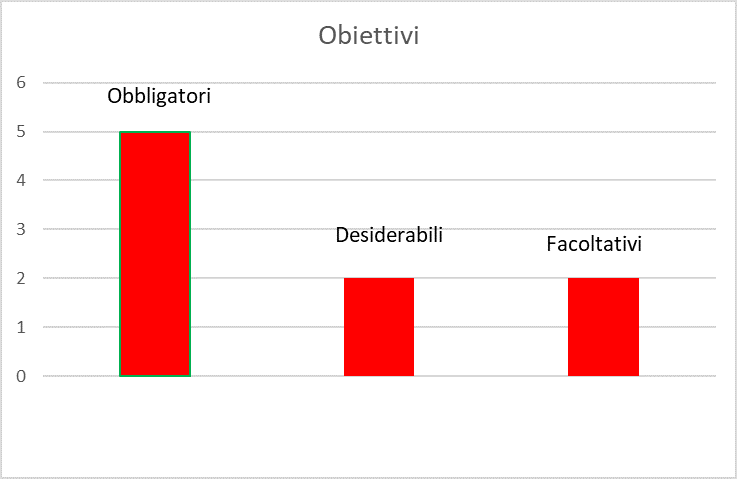
\includegraphics[width=9cm]{immagini/requisiti2.png}
	\centering
	\caption{Requisiti}
\end{figure}


\subsection{Requisiti obbligatori}
\begin{itemize}
	\item Ottimizzazione della pianificazione tenendo conto delle giacenze
	di magazzino: raggiungimento totale;
	\item Sviluppo di nuove strategie di scelta dell’Algoritmo Greedy e
	confronto dei risultati ottenuti in relazione alla funzione obiettivo: raggiungimento totale;
	\item Integrazione della Tabu Search con nuovi criteri di aspirazione e
	arresto: raggiungimento totale;
	\item Sviluppo di nuovi meccanismi di esplorazione del vicinato nella
	Tabu Search: raggiungimento totale;
	\item Acquisizione di competenze sull’utilizzo di algoritmi di Ricerca
	Operativa e applicazione in un caso di studio reale: raggiungimento totale.

	
\end{itemize}

\subsection{Requisiti desiderabili}
\begin{itemize}
	\item Ottimizzazione della pianificazione tenendo conto degli ordini a
	fornitore presenti a sistema: raggiungimento totale;
	\item Ottimizzazione della pianificazione tenendo conto dei
	semilavorati: raggiungimento totale;
\end{itemize}

\subsection{Requisiti opzionali}
\begin{itemize}
	\item Utilizzo di multithreading nelle fasi in cui è richiesta una maggiore
	capacità di calcolo: raggiungimento totale;
	\item Data una pianificazione inserita a sistema, eseguire una
	ripianificazione considerando vincoli dovuti a necessità aziendali
	dell’ultimo momento (anomalie, guasti, ordini urgenti, etc.): raggiungimento nullo.
\end{itemize}

Come accennato nella sezione precedente il requisito FA2 "Data una pianificazione inserita a sistema, eseguire una
ripianificazione considerando vincoli dovuti a necessità aziendali
dell’ultimo momento" è stato scartato a seguito di una riunione con il tutor aziendale. Siamo quindi giunti alla conclusione che, in termini di efficacia, è preferibile una nuova esecuzione dell'algoritmo a partire da zero piuttosto che conservare gli attuali dati e procedere con una nuova rielaborazione. Questo rende anche più facile la definizione e l'aggiunta dei nuovi vincoli imposti, quali linee bloccate o sequenze non più attive, che potrebbero influenzare negativamente i precedenti dati inseriti.


\section{Divisione settimanale}

La seguente sezione vuole descrivere come sono state suddivise le 320 ore previste per il periodo di stage, affiancando ad ogni settimana lavorativa i requisiti e gli obiettivi raggiunti. Il periodo di stage inizia in data 09-settembre-2019 con termine ufficiale in data 01-novembre-2019 traslata al 03-novembre-2019 a causa del sostenimento di due prove d'esame.

\begin{itemize}
	\item \textbf{Prima settimana}:
	\begin{itemize}
		 \item analisi del modulo software esistente;
		 \item funzionalità da realizzare;
	 	 \item studio della documentazione disponibile dell’algoritmo esistente.
	\end{itemize}
	\item \textbf{Seconda settimana}: 
	\begin{itemize}
		\item analisi dei rischi;
		\item stesura dell'analisi dei requisiti che comprende le nuove funzionalità da integrare nel software esistente;
		\item  inizio della stesura di documentazione a supporto dell'architettura utilizzata.
	\end{itemize}
	\item \textbf{Terza settimana}:
		\begin{itemize}
		\item Studio delle tecnologie aziendali necessarie allo sviluppo del
		modulo in particolare linguaggio di programmazione VB.NET\glo, componenti
		DevExpress\glosp e database Informix\glo;
		\item  training\glosp sulle nuove tecnologie da utilizzare con realizzazione di un software di prova;
		\item studio di algoritmi e tecniche di Ricerca Operativa e	Ottimizzazione Combinatoria;
		\item riunioni col tutor aziendale per decidere le scelte implementative dell'algoritmo Greedy.
	\end{itemize}
	\item \textbf{Quarta settimana}:
		\begin{itemize}
		\item Algoritmo Greedy: sviluppo di nuove strategie di scelta
		del passo successivo adottato dall’algoritmo nella
		costruzione della soluzione del problema;
		\item sviluppo procedura di gestione delle giacenze di
		magazzino.
		\end{itemize}
	\item \textbf{Quinta settimana}:
		\begin{itemize}
		\item sviluppo procedura di gestione dei semilavorati
		pianificati;
			\item sviluppo procedura di gestione degli ordini fornitori.
		\end{itemize}
	\item \textbf{Sesta settimana}:
		\begin{itemize}
		\item integrazione della Tabu Search con nuovi meccanismi:
		criteri di aspirazione e arresto, variazione dei
		meccanismi di esplorazione del vicinato e adozione di
		tecniche di intensificazione e diversificazione.
		\end{itemize}
	\item \textbf{Settima settimana}:
		\begin{itemize}
		\item fase di test dei dati con valori reali forniti dai clienti di Ergon;
		\item comparazione dell'algoritmo ultimato con il precedente algoritmo in uso;
		\item verifica della bontà della soluzione in rapporto coi dati forniti dai clienti.
		\end{itemize}
	\item \textbf{Ottava settimana}:
		\begin{itemize}
		\item stesura della documentazione a supporto del prodotto sviluppato, con risalto sulle scelte implementative non banali.
		\end{itemize}
\end{itemize}

Da sottolineare il fatto che le fasi di test sono state molteplici e non solo durante la settima settimana. Ad ogni nuova aggiunta veniva effettuato un controllo sul risultato prodotto dalla pianificazione con dei dati reali di supporto, tutto ciò per garantire la correttezza della logica del codice in aggiunta. In comune accordo con il tutor abbiamo deciso di iniziare dalle parti più complesse la nuova fase di implementazione, così da garantire una continua verifica ad ogni aggiunta delle funzionalità meno importanti.

\pagebreak
\section{Analisi dei rischi}
Ho trovato importante individuare eventuali rischi che possono portare a problematiche in grado di far procedere a rilento la realizzazione del progetto di stage.
Di seguito viene presentata la tabella contenente i rischi preventivati durante la seconda settimana di stage. Ogni rischio possiede un codice identificativo, una breve descrizione affiancata dal suo rilevamento e relativo grado di rischio. Per ogni rischio è definito inoltre un piano di contingenza da seguire in caso di occorrenza del rischio.



\renewcommand{\arraystretch}{1.5}
\rowcolors{2}{dispari}{pari}
\arrayrulecolor{white}
\begin{longtable}{ 
		>{\centering}p{0.17\textwidth} 
		>{\raggedright}p{0.28\textwidth}
		>{\raggedright}p{0.29\textwidth} 
		>{\centering}p{0.15\textwidth}
	}
	
	\caption{Tabella dei rischi di progetto}\\
	\rowcolorhead
	\colorhead\textbf{Codice \\ Nome} & \centering\colorhead\textbf{Descrizione} & 
	\centering\colorhead\textbf{Piano di contingenza} & 
	\colorhead\textbf{Grado di rischio} 
	\tabularnewline
	\endfirsthead
	\rowcolor{white}\caption[]{(continua)}\\
	\rowcolorhead
	\colorhead\textbf{Nome \\ Codice} & \centering\colorhead\textbf{Descrizione} & 
	\centering\colorhead\textbf{Rilevamento} & 
	\colorhead\textbf{Grado di rischio} 
	\tabularnewline
	\endhead
	
	%RO1---------------------------------------------------------
	\rowcolordark \textbf{RO1} \\ Problematiche di Ricerca Operativa & 
	Dovendo svolgere uno studio individuale delle tematiche di Ricerca Operativa da affrontare, è possibile imbattersi in argomenti poco intuitivi o complicati da apprendere in solitaria. &
	Vengono fornite le dispense riguardanti il contesto in cui si andrà a lavorare e in caso di incomprensioni si farà affidamento sia sul tutor interno sia al proprio relatore. &
	Occorrenza: \textbf{Media} \\
	Pericolosità: \textbf{Alta} 
	\tabularnewline
	
	%RT1---------------------------------------------------------
	\rowcolorlight \textbf{RT1} \\ Inesperienza tecnologica & 
	Alcune delle tecnologie adottate sono nuove, pertanto è possibile incorrere in problemi durante lo svolgimento delle attività che le coinvolgono. &
	Viene fornita la documentazione ufficiale in modo da avere ampio supporto per qualsiasi lacuna di natura tecnica. Se ciò non dovesse bastare si farà affidamento al tutor interno o qualche membro delegato del team di sviluppo di Ergon. &
	Occorrenza: \textbf{Media} \\
	Pericolosità: \textbf{Media} 
	\tabularnewline

	%RT2---------------------------------------------------------
	\rowcolordark \textbf{RT2} \\ Scelte implementative & 
	Non è detto che tutte le scelte prese in considerazione durante lo studio del problema portino ad una corretta soluzione o ad una esecuzione in tempi accettabili. &
	Verranno valutate, in caso di necessità, nuove strade da percorrere per la risoluzione del problema. &
	Occorrenza: \textbf{Bassa} \\
	Pericolosità: \textbf{Alta} 
	\tabularnewline
	
	
\end{longtable}
	
\renewcommand{\arraystretch}{1}             % Processi
% !TEX encoding = UTF-8
% !TEX TS-program = pdflatex
% !TEX root = ../tesi.tex

%**************************************************************
\chapter{Analisi del problema e studio delle tecnologie}
\label{cap:progetto-stage}
%**************************************************************

\section{Specifiche tecniche del problema}

Nel primo periodo di stage, il tempo è stato dedicato allo studio delle componenti del problema da affrontare, ricavando un quadro generale del
funzionamento logico della pianificazione della produzione. 
Perché un prodotto venga pianificato, è necessario che ci sia almeno una linea in grado di produrlo, una volta definita la linea si deve scegliere una sequenza in 
cui produrre l'articolo. Una sequenza definisce giorno, data di inizio e di fine e può comprendere un insieme di vincoli da soddisfare
(quali lavaggi oppure ordinaria manutenzione), l'articolo verrà quindi inserito all'interno della sequenza con il relativo tempo di produzione.
Ogni linea ha solitamente più sequenze, nelle quali è possibile collocare l'articolo. Ogni sequenza può avere dei vincoli di dipendenza con altre sequenze.


\subsection{Implementazione}
Segue la descrizione della struttura, ad alto livello, riguardante le principali meccaniche che rientrano nell'uso dell'applicativo.

\subsubsection{Linee}
Indica l'insieme delle linee sulle quali è consentita la produzione degli ordini, ogni linea ha relativo costo orario e definisce l'insieme degli articoli che può produrre con annessa velocità di produzione.
Ogni linea è così definita:
\begin{itemize}
	\item \textbf{Codice Linea}: serve ad indicare su quale linea si vuole produrre l'articolo;
	\item \textbf{Info Articolo}: lista che indica quali articoli la linea può produrre con relativo tempo di produzione;
	\item \textbf{Info Vincolo}: lista che indica i vincoli presenti sulla linea, possono essere obbligatori o opzionali;
	
	\item \textbf{Sequenze Linea}: lista che indica quali sono le sequenze di produzione della linea;
	
	\item \textbf{Pianificazione}: lista che indica quali articoli e quali vincoli sono stati pianificati nella linea corrente;
	
	
	\item \textbf{Errori}: indica quali errori si sono presentati durante la pianificazione;
	
	\item \textbf{Calendario}: indica quali sono i giorni lavorativi con le eventuali pause.
	
\end{itemize}

\subsubsection{Sequenze}
Indica l'insieme delle sequenze di produzione presenti su ogni linea, nelle quali vengono inseriti gli ordini che sono stati pianificati.
Ogni sequenza è così definita:
\begin{itemize}
	\item \textbf{Codice Sequenza}: serve ad indicare su quale sequenza si vuole inserire l'articolo;
	\item \textbf{Giorno}: indica il giorno nel quale si vuole inserire l'articolo;
	\item \textbf{Ora inizio/Ora fine}: indica gli orari di inizio e fine della sequenza corrente;
	
	\item \textbf{Elementi}: lista che indica gli articoli e i vincoli appartenenti alla sequenza corrente.
	
\end{itemize}

\subsubsection{Ordine}
Indica come si presenta un ordine da produrre.
Ogni ordine è così definito:
\begin{itemize}
	\item \textbf{Codice Articolo}: indica il codice dell'articolo;
	\item \textbf{Tipo Articolo}: indica il tipo dell'articolo, può essere un prodotto finito, semilavorato o materia prima;
	\item \textbf{Codice Linea}: indica il livello più generale della gerarchia di classificazione di un prodotto;
	\item \textbf{Codice Settore}: indica il terzo livello di gerarchia di classificazione;
	\item \textbf{Codice Famiglia}: indica il secondo livello di gerarchia, definisce la famiglia del prodotto;
	\item \textbf{Codice SottoFamiglia}: indica il livello più caratterizzante della classificazione di un prodotto;
	
	\item \textbf{Quantità}: indica la quantità richiesta da produrre;
	
	\item \textbf{Data Spedizione}: indica la data di spedizione dell'articolo;
	
	\item \textbf{Ora spedizione}: indica l'ora di spedizione dell'articolo;
	
	\item \textbf{Data Consegna}: indica la data di consegna presso la sede del cliente;
	 
	\item \textbf{Linea preferenziale}: indica la linea preferenziale di produzione dell'articolo;
	
	\item \textbf{Anno Ordine}: indica l'anno dell'ordine in questione; 

    \item \textbf{Materie Prime}: lista che indica l'insieme delle materie prime richieste per la produzione dell'ordine;
  
   \item \textbf{Semilavorati}: lista che indica l'insieme dei semilavorati richiesti per la produzione dell'ordine;
   
   \item \textbf{Riferimento Ordine}: lista che indica l'insieme degli ordini ai quali l'ordine corrente fa riferimento per la produzione di semilavorati;
   
\end{itemize}

\subsection{Problemi logici da affrontare}
Di seguito sono presentate le problematiche che l'algoritmo deve affrontare per ottenere una corretta pianificazione della produzione.

\subsubsection{Temporali}
I problemi riguardanti i tempi di produzione sono legati a:
\begin{itemize}
	\item \textbf{Data Spedizione}: devono essere rispettate le date di spedizione e di consegna degli articoli da pianificare;
	\item \textbf{Tempo minimo alla consegna}: devono essere rispettate le date di inizio produzione nel caso di ordini con scadenza a breve termine;
	
	\item \textbf{Semilavorati}: i semilavorati di un ordine devono essere pianificati prima dell'ordine stesso;
	
	\item \textbf{Ordini Fornitori}: vanno considerate le date di arrivo delle materie prime da parte dei fornitori in modo da non scartare la produzione di ordini che sarebbero producibili;
	
	\item \textbf{Giorni Lavorativi}: devono essere rispettati i giorni lavorativi senza pianificare ordini al di fuori di essi;
	\item \textbf{Orario Lavorativo}: devono essere rispettati gli orari lavorativi senza eccedere dal monte ore impostato dall'azienda che esegue la pianificazione;
	\item \textbf{Sovrapposizione Sequenze}: ogni linea può produrre una singola sequenza per volta;	
	\item \textbf{Sovrapposizione Articoli}: ogni sequenza può contenere un solo articolo senza sovrapporne degli altri nello stesso lasso di tempo.
\end{itemize}

\subsubsection{Vincoli}
I vincoli da rispettare sono:
\begin{itemize}
	
	\item \textbf{Materie prime}: non è possibile produrre un ordine se non sono presenti sufficienti materie prime;
	
	\item \textbf{Vincoli Obbligatori}: devono essere pianificati tutti i vincoli obbligatori di ogni sequenza;
	\item \textbf{Vincoli Condizionati}: devono essere pianificati tutti i vincoli condizionati di ogni sequenza in base alle condizioni imposte;
\item \textbf{Vincoli Opzionali}: devono essere pianificati i vincoli opzionali solo in caso ci sia una finestra temporale sufficiente altrimenti si lascia spazio alla produzione di articoli;
	\item \textbf{Vincoli Articolo}: devono essere rispettati i vincoli di produzione di ogni articolo, quali linea preferenziale o linea con maggiore velocità di produzione.
\end{itemize}

\subsubsection{Scelte implementative}
Dopo una discussione col tutor interno abbiamo scartato l'ultimo vincolo facoltativo FA2, presente nel piano di lavoro, il quale riguardava la ripianificazione
degli articoli in caso di guasti o necessità aziendali, optando per una semplice nuova esecuzione dell'applicativo con i nuovi dati interessati. 



\section{Analisi dei requisiti}

Uno dei requisiti vincolava la modifica a livello grafico dell'applicativo, in quanto la clientela era abituata alla versione corrente e non sempre
è immediato adattarsi a cambiamenti di questo tipo.\\ 
Si è quindi fatto affidamento all'analisi dei requisiti stilata dallo stagista precedente \hyperref[analisi-requisiti]{[3]}.
Sono stati aggiunti due casi particolari che verranno evidenziati di seguito.

%************************************************************

\subsection{Casi d'uso}

Per rappresentare l'insieme delle azioni comuni ad un singolo utente sono stati utilizzati i casi d'uso.
Per descrivere i vari scenari ho mantenuto la precedente scaletta di informazioni così da dare una continuità al documento esistente. 
Ciascun caso d'uso sarà quindi rappresentato come descritto di seguito:
\begin{itemize}
    \item \textbf{Identificatore} univo nel formato UC-[Codice];
    \item \textbf{Titolo} del caso d'uso;
    \item \textbf{Descrizione} generale del caso d'uso;
    \item \textbf{Attori} coinvolti: primari e secondari;
    \item \textbf{Precondizione} del caso d'uso;
    \item \textbf{Scenario principale} che il caso d'uso vuole modellare, identificando ogni azione che ne fa parte;
    \item \textbf{Postcondizione} del caso d'uso;
    \item \textbf{Estensioni} dello scenario principale, evidenziata da una lettera maiuscola e inserita in un elenco.
\end{itemize}

Di seguito vengono rappresentate le modifiche apportate al documento esistente\hyperref[analisi-requisiti]{\textsuperscript{3}}.
Si fa riferimento allo standard UML 2.0\hyperref[uml]{[4]} per la rappresentazione dei casi d'uso.

\subsection*{UC-3 Pianificazione della produzione}

\begin{figure}[H]
	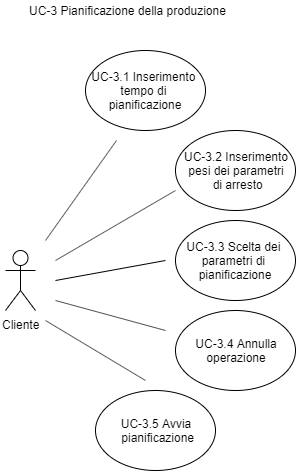
\includegraphics[width=8cm]{immagini/UC1.png}
	\centering
	\caption{Use Case - UC-3}
\end{figure}

\textbf{Attori}: Cliente. \newline
\textbf{Descrizione}: Il cliente esegue la pianificazione degli ordini selezionati.\newline
\textbf{Precondizione}: Il cliente ha selezionato gli ordini che intende pianificare e i giorni in cui vuole farlo.\newline
\textbf{Scenario principale}: \begin{itemize}
    \item Il cliente seleziona che ordini vuole pianificare;
    \item Il cliente preme il pulsante "Pianifica";
    \item Il cliente modifica i parametri della pianificazione come previsto dagli UC-3.1, UC-3.2, UC-3.3;
    \item Il cliente preme il pulsante "Avvia pianificazione".
\end{itemize}

\textbf{Postcondizione}: Nella finestra principale viene visualizzato il risultato della pianificazione.


\subsection*{UC-3.3 Scelta dei parametri di pianificazione}

\begin{figure}[H]
	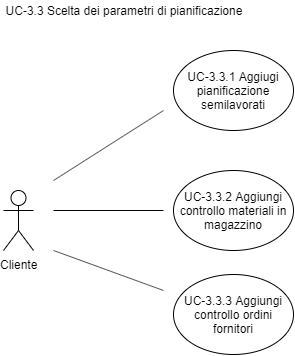
\includegraphics[width=8cm]{immagini/UC2.png}
	\centering
	\caption{Use Case - UC-3.3}
\end{figure}

\textbf{Attori}: Cliente. \newline
\textbf{Descrizione}: Il cliente seglie i parametri da considerare nella pianificazione.\newline
\textbf{Precondizione}: Il cliente ha selezionato il pulsante "Metodo di pianificazione".\newline
\textbf{Scenario principale}: \begin{itemize}
    \item Il cliente seleziona come effettuare le pianificazione;
    \item Il cliente può selezionare le varie aggiunte descritte dagli UC-3.3.1, UC-3.3.2, UC3.3.3;
    \item Il cliente preme il pulsante "Conferma".
\end{itemize}
\textbf{Postcondizione}: Si verrà ricondotti allo use case UC-3.3.
\newpage
\section{Tracciamento dei requisiti}

Ogni requisito è composto dalla seguente struttura:
\begin{itemize}
	\item \textbf{codice identificativo}: ogni codice identificativo è univoco e conforme alla seguente codifica:\\
	\centerline{\textbf{RE[Importanza][Tipologia][Codice]}} \\ \\
	Il significato delle cui voci è:
	\begin{itemize}
		\item \textbf{Tipologia}: ogni requisito può assumere uno dei seguenti valori:
		\begin{itemize}
			\item \textit{F}: funzionale;
			\item \textit{P}: prestazionale;
			\item \textit{Q}: qualitativo;
			\item \textit{V}: vincolo.
		\end{itemize}
		\item \textbf{Importanza}: ogni requisito può assumere uno dei seguenti valori:
		\begin{itemize}
			\item \textit{O}: requisito obbligatorio: irrinunciabili per qualcuno degli stakeholder;
			\item \textit{D}: requisito desiderabile: non strettamente necessari ma  a valore aggiunto riconoscibile;
			\item \textit{F}: requisito facoltativo: relativamente utili oppure contrattabili più avanti nel progetto.	
		\end{itemize}
		\item \textbf{Codice}: è un identificatore univoco del requisito segue un ordine incrementale.
	\end{itemize}
	\item \textbf{classificazione}: viene riportata l'importanza del requisito. Sebbene questa sia un'informazione ridondante ne facilita la lettura;
	\item \textbf{descrizione}: descrizione breve ma completa del requisito, meno ambigua possibile.
\end{itemize}
\renewcommand{\arraystretch}{1.5}



\subsection{Requisiti funzionali}

L'insieme delle funzionalità che il sistema deve fornire vengono definite nella \hyperref[3.1]{Tabella 3.1}.

\renewcommand{\arraystretch}{1.5}
\rowcolors{2}{dispari}{pari}
\arrayrulecolor{white}

\begin{longtable}{ >{\centering}p{0.15\textwidth} >{\centering}p{0.20\textwidth}
		>{\raggedright}p{0.35\textwidth} >{\centering}p{0.14\textwidth}}
	\caption{Tabella dei requisiti funzionali}
	\label{3.1}
	\\
	\rowcolorhead 
	\textbf{\color{white}Requisito} 
	& \textbf{\color{white}Classificazione} 
	& \centering\textbf{\color{white}Descrizione}
	 
	\endfirsthead
	\rowcolor{white}\caption[]{(continua)}\\
	\rowcolorhead 
	\textbf{\color{white}Requisito} 
	& \textbf{\color{white}Classificazione} 
	& \centering\textbf{\color{white}Descrizione}
	
	\endhead	
	
	REFO1	&	Obbligatorio	&	Il sistema permette l’inserimento di un nuovo vincolo di linea	 \tabularnewline
	REFO2	&	Obbligatorio	&	Il sistema permette la modifica dei dati di un vincolo di linea esistente	\tabularnewline
	REFO3	&	Obbligatorio	&	Il sistema permette l’eliminazione di un vincolo di linea 	\tabularnewline
	REFO4	&	Obbligatorio	&	L’interfaccia permette l’eliminazione di una linea 	\tabularnewline
	REFO5	&	Obbligatorio	&	 Il sistema permette l’aggiunta di una nuova sequenza	\tabularnewline
	REFO6	&	Obbligatorio	&	 Il sistema permette la modifica dei dati di una sequenza esistente	\tabularnewline
	REFO7	&	Obbligatorio	&	 Il sistema permette l’eliminazione di un articolo di sequenza esistente	\tabularnewline
	REFO8	&	Obbligatorio	&	 Il sistema permette l’eliminazione di un vincolo di sequenza esistente	\tabularnewline
	REFO9	&	Obbligatorio	&	 Il sistema permette l’eliminazione di una sequenza	\tabularnewline
	REFO10	&	Obbligatorio	&	 Il sistema permette all’utente di scegliere un tempo massimo di esecuzione dell’algoritmo	\tabularnewline
	REFO11	&	Obbligatorio	&	 Il sistema permette all’utente di assegnare un peso all’importanza di parametri di produzione quali:pezzi prodotti e occupazione delle linee	\tabularnewline
	REFD1	&	Desiderabile	&	 Il sistema permette all’utente di scegliere se ricalcolare la pianificazione già esistente	\tabularnewline
	REO12	&	Obbligatorio	&	 Il sistema permette di pianificare automaticamente la produzione dato un insieme di ordini e un intervallo di tempo	\tabularnewline
	REFO1	&	Obbligatorio	&	 Il sistema permette di scegliere i relativi criteri di pianificazione	\tabularnewline
\end{longtable}

\newpage
\subsection{Requisiti qualitativi}

Vengono illustrati nella \hyperref[3.2]{Tabella 3.2} i requisiti che incrementano la qualità generale del sistema.

\rowcolors{2}{pari}{dispari}

\begin{longtable}{ >{\centering}p{0.15\textwidth} >{\centering}p{0.20\textwidth}
		>{\raggedright}p{0.35\textwidth} >{\centering}p{0.14\textwidth}}
	\caption{Tabella dei requisiti qualitativi}
	\label{3.2}
	\\
	\rowcolorhead 
	\textbf{\color{white}Requisito} 
	& \textbf{\color{white}Classificazione} 
	& \centering\textbf{\color{white}Descrizione}
	 
	\endfirsthead
	\rowcolor{white}\caption[]{(continua)}\\
	\rowcolorhead 
	\textbf{\color{white}Requisito} 
	& \textbf{\color{white}Classificazione} 
	& \centering\textbf{\color{white}Descrizione}
	
	\endhead	
	
	REQD1	&	Desiderabile	&	Il programma genera un file di \hyperref[Log]{Log\glo} di supporto al \hyperref[Debug]{Debug\glo}	 \tabularnewline
	REQO1	&	Obbligatorio	&	Ogni scelta non banale effettuata è adeguatamente commentata nel codice	\tabularnewline
	REQF1	&	Facoltativo		&	Fornire un manuale utente	\tabularnewline
	REQF2	&	Facoltativo		&	Fornire un manuale sviluppatore	\tabularnewline

\end{longtable}

\subsection{Requisiti prestazionali}

La \hyperref[3.3]{Tabella 3.3} definisce i requisiti riguardanti le prestazioni attese dal software.

\rowcolors{2}{pari}{dispari}

\begin{longtable}{ >{\centering}p{0.15\textwidth} >{\centering}p{0.20\textwidth}
		>{\raggedright}p{0.35\textwidth} >{\centering}p{0.14\textwidth}}
	\caption{Tabella dei requisiti prestazionali}
	\label{3.3}
	\\
	\rowcolorhead 
	\textbf{\color{white}Requisito} 
	& \textbf{\color{white}Classificazione} 
	& \centering\textbf{\color{white}Descrizione}
	 
	\endfirsthead
	\rowcolor{white}\caption[]{(continua)}\\
	\rowcolorhead 
	\textbf{\color{white}Requisito} 
	& \textbf{\color{white}Classificazione} 
	& \centering\textbf{\color{white}Descrizione}
	
	\endhead	
	
	REPD1	&	Desiderabile	&	L'applicativo deve fornire una soluzione entro il tempo stabilito dall'utente	 \tabularnewline
	REPD2	&	Desiderabile	&	L'applicativo deve fornire la soluzione nel modo più rapido possibile senza valutare ulteriori combinazioni se è stato
	raggiunto un determinato punteggio stabilito per la soluzione stessa \tabularnewline
	REPD3	&	Desiderabile	&	La fase di lettura dei dati deve essere eseguita in tempi inferiori ai 30 minuti \tabularnewline

\end{longtable}
\newpage
\subsection{Requisiti vincolo}

La \hyperref[3.4]{Tabella 3.4} definisce i requisiti vincolanti per l'integrazione di nuove componenti nel sistema preesistente.

\rowcolors{2}{pari}{dispari}

\begin{longtable}{ >{\centering}p{0.15\textwidth} >{\centering}p{0.20\textwidth}
		>{\raggedright}p{0.35\textwidth} >{\centering}p{0.14\textwidth}}
	\caption{Tabella dei requisiti prestazionali}
	\label{3.4}
	\\
	\rowcolorhead 
	\textbf{\color{white}Requisito} 
	& \textbf{\color{white}Classificazione} 
	& \centering\textbf{\color{white}Descrizione}
	 
	\endfirsthead
	\rowcolor{white}\caption[]{(continua)}\\
	\rowcolorhead 
	\textbf{\color{white}Requisito} 
	& \textbf{\color{white}Classificazione} 
	& \centering\textbf{\color{white}Descrizione}
	
	\endhead	
	
	REVO1	&	Desiderabile	&    Rendere compatibile il programma con l’attualemodulo di pianificazione della produzione	 \tabularnewline
	REVO2	&	Desiderabile	&    Ottimizzare la pianificazione tenendo conto delle materie prime e dei semilavorati	 \tabularnewline
	REVO3	&	Desiderabile	&    Ottimizzare la pianificazione tenendo conto degli ordini dei fornitori inseriti a sistema	 \tabularnewline
	REVO4	&	Desiderabile	&    Ottimizzare la pianificazione rendendo possibile la pianificazione dei semilavorati	 \tabularnewline
	REVO5	&	Desiderabile	&    Il programma è sviluppato tramite il linguaggio diprogrammazione Vb.NET v.4.7.0	 \tabularnewline
	REVO6	&	Desiderabile	&    \hyperref[IDE]{L’IDE\glo} (Integrated development environment) utilizzato è Microsoft Visual Studio v.10.0.4	 \tabularnewline
	REVO7	&	Desiderabile	&    Le componenti grafiche sono basate sulle DevEx-press	 \tabularnewline
	REVO8	&	Desiderabile	&    I dati vengono salvati su un database Informix	 \tabularnewline
	REVO9	&	Desiderabile	&    I dati in input sono scritti su un file JSON	 \tabularnewline
	REVO10	&	Desiderabile	&    I dati in output sono scritti su un file JSON	 \tabularnewline

\end{longtable}

\newpage
\subsection{Riepilogo dei requisiti}

La \hyperref[3.5]{Tabella 3.5} riassume l'insieme dei requisiti che il sistema deve soddisfare.

\rowcolors{2}{pari}{dispari}

\begin{longtable}{ >{\centering}p{0.15\textwidth} >{\centering}p{0.20\textwidth}
		>{\centering}p{0.35\textwidth} >{\centering}p{0.14\textwidth}}
	\caption{Tabella del riepilogo dei requisiti}
	\label{3.5}
	\\
	\rowcolorhead 
	\textbf{\color{white}Tipo} 
	& \textbf{\color{white}Obbligatori} 
	& \centering\textbf{\color{white}Desiderabili}
	& \centering\textbf{\color{white}Facoltativi}
	
	\endhead	
	
	Funzionali	&	13	&  1  &	0 \tabularnewline
	Qualitativi	&	1	&  1  &	 2 \tabularnewline
	Prestazionali	&	0	&   3 & 0	 \tabularnewline
	Di vincolo	&	10	& 0   &	0 \tabularnewline
	Totali	&	24	&   5 &	2 \tabularnewline

\end{longtable}
\newpage
\section{Tecnologie e strumenti}

Di seguito sono riportate tutte le tecnologie utilizzate durante lo sviluppo del progetto.
Tali scelte sono state imposte da Ergon Informatica in quanto sono gli strumenti che vengono utilizzati dall'azienda per lo sviluppo dei progetti interni.\\
La scelta è inoltre guidata dal fatto che, per mantenere l'integrazione con le parti già esistenti dell'applicativo e il suo funzionamento tramite il software Ergdis, 
non è stato possibile spostarsi su nuove tecnologie, magari anche solo a qualche versione successiva di esse.\\
Ergon Informatica si appoggia a questi strumenti in quanto sono forniti di un ottima documentazione di supporto, hanno un alto tasso di scalabilità 
e forniscono un supporto in tempo reale alla codifica.\\ \\

\textbf{Vb.NET}

Vb.NET, il cui logo è mostrato in \hyperref[net]{Figura 3.3}, è linguaggio di programmazione che deriva da Visual Basic 6,
 è sviluppato da Microsoft e, al contrario dei precedenti, supporta il paradigma di programmazione
orientata agli oggetti \hyperref[vbnet]{[5]}.

\begin{figure}[H]
	
\includegraphics[width=5cm]{immagini/vb.png}
	\centering
	\caption{Logo Vb.NET\hyperref[vb-logo]{[6]}}
	\label{net}
\end{figure}

Vb.NET consente lo sviluppo di applicazioni Windows, Web e per dispositivi mobili. \\
Come avviene con tutti i linguaggi basati su Microsoft .NET Framework,
i programmi scritti in Vb.NET usufruiscono delle funzionalità di sicurezza e interoperabilità dei linguaggi.\\
Nel progetto viene utilizzato questo linguaggio per poter usufruire delle classi, le quali riducono significativamente le duplicazioni di codice e rendono l'intero sorgente 
chiuso alle modifiche e aperto agli ampliamenti. \\Viene inoltre utilizzato in quanto è il linguaggio attualmente adottato dall'azienda per lo sviluppo e si presta bene
al tipo di lavorazioni necessarie a portare a compimento lo sviluppo dell'applicativo.

\newpage
\textbf{Visual Studio 2010}\\
Visual Studio 2010, il cui logo è mostrato in \hyperref[vs-2010]{Figura 3.4}, è un ambiente di sviluppo integrato sviluppato da Microsoft \hyperref[vs]{[7]}. 
\begin{figure}[H]
	
\includegraphics[width=9cm]{immagini/microsoft-visual-studio-2010-logo.png}
	\centering
	\caption{Logo Visuali Studio 2010\hyperref[vs-logo]{[8]}}
	\label{vs-2010}
\end{figure}


La prima versione risale al 1997 con lo scopo di fornire
un ambiente di sviluppo grafico ed integrato che aiutasse lo sviluppatore a gestire i progetti in maniera semplice, ma efficace, aumentandone quindi la produttività.\\
Microsoft ha incluso il supporto a differenti linguaggi di programmazione.\\
In Ergon Informatica è il principale ambiente di sviluppo sia per applicazioni desktop che mobile, di conseguenza è stato utilizzato anche durante lo sviluppo del progetto.\\

\textbf{DevExpress}\\

\textit{Developer Express Inc.}, il cui logo è mostrato in \hyperref[dev-exp]{Figura 3.5}, è una società di sviluppo software fondata nel 1998, inizialmente fornisce un insieme di controlli 
\hyperref[UI]{UI\glo} poi sviluppa diverse estensioni per le librerie grafiche \hyperref[devexpress]{[9]}.

\begin{figure}[H]
	\includegraphics[width=8cm]{immagini/devexpress.png}
	\centering
	\caption{Logo DevExpress\hyperref[devlogo]{[10]}}
	\label{dev-exp}
\end{figure}

In particolare nel progetto ci si è appoggiati a questa tecnologia per velocizzare la creazione dell'interfaccia grafica sulla quale si basa il modo di rappresentare la soluzione
che viene fornita, permettendo una chiara visualizzazione tabellare grazie ad una delle tante \hyperref[Estensioni]{estensioni\glo} utilizzabili. 

\newpage

\textbf{JSON}

Acronimo di \textit{JavaScript Object Notation}, il cui logo è mostrato in \hyperref[js]{Figura 3.6}, è un formato adatto
all'interscambio di dati fra applicazioni \hyperref[Client/Server]{client/server\glo} \hyperref[json]{[11]}.

\begin{figure}[H]
	
\includegraphics[width=3cm]{immagini/json.png}
	\centering
	\caption{Logo JSON\hyperref[jlogo]{[12]}}
	\label{js}
\end{figure}

Serve, in particolare, a fornire una struttura a dati interessati rendendoli interscambiabili tra diverse applicazioni senza che si renda necessaria la codifica e decodifica di quest'ultimi.
Nel nostro caso si rende utile quando è necessario delegare l'esecuzione di operazioni sui dati prelavati da un terminale con accesso al database verso un terminale esterno.
I dati raccolti dal database venivano trasferiti in un file JSON, il quale veniva inviato al successivo passo di esecuzione dell'algoritmo, al termine di ciò veniva restituita
la soluzione sempre in formato JSON a chi ne aveva fatto richiesta e di conseguenza visualizzata.\\

\textbf{Informix}

Informix, il cui logo è mostrato in \hyperref[ibm]{Figura 3.7}, fa parte della divisione \hyperref[DBMS]{DBMS\glo} (Database Management System) di IBM, è un sistema software progettato per consentire la creazione,
la manipolazione e l'interrogazione efficiente di database \hyperref[informix]{[13]}.

\begin{figure}[H]
	\includegraphics[width=7cm]{immagini/Informix.png}
	\centering
	\caption{Logo Informix\hyperref[ilogo]{[14]}}
	\label{ibm}
\end{figure}


L'Informix server supporta il modello relazionale ad oggetti che permette ad IBM di offrire estensioni che supportano i tipi di dati che non sono una parte dello standard SQL.
Le estensioni più usate sono quelle riguardanti le serie temporali e spaziale che forniscono entrambe supporto al tipo di dato ed estensioni linguistiche che permettono 
interrogazioni per un dominio specifico ad alte prestazioni e archiviazione efficiente per set di dati basati su serie temporali e dati spaziali.
È il servizio database sul quale fa affidamento l'azienda, essendo IBM uno dei partner principali di Ergon Informatica.             % Kick-Off
% !TEX encoding = UTF-8
% !TEX TS-program = pdflatex
% !TEX root = ../tesi.tex

%**************************************************************
\chapter{Progettazione e sviluppo}
\label{cap:progettazione}
%**************************************************************

\section{Progettazione}
\subsection{Architettura}

Prima di descrivere la varie aggiunte che sono state apportate al software, è necessario fornire un'idea dell'architettura sulla quale il progetto si basa. In questo modo si 
rendono più chiare molte delle scelte che sono state prese e il perché altre sono state scartate.\\ Di seguito è presentato uno schema ad alto livello di come sono strutturate le
varie componenti che formano l'intero sistema. Come possiamo notare in \hyperref[4.1]{Figura 4.1}, il progetto segue un flusso pressoché "ciclico", partendo dal recupero dei dati dal
database e infine fornendo la soluzione. I dati estratti dal database vengono convertiti in file JSON il quale verrà letto dall'algoritmo che ha il compito di trovare la soluzione,
una volta fornita la soluzione essa viene ritradotta in un file JSON il quale viene letto e trasposto nell'interfaccia utente.

\begin{figure}[H]
	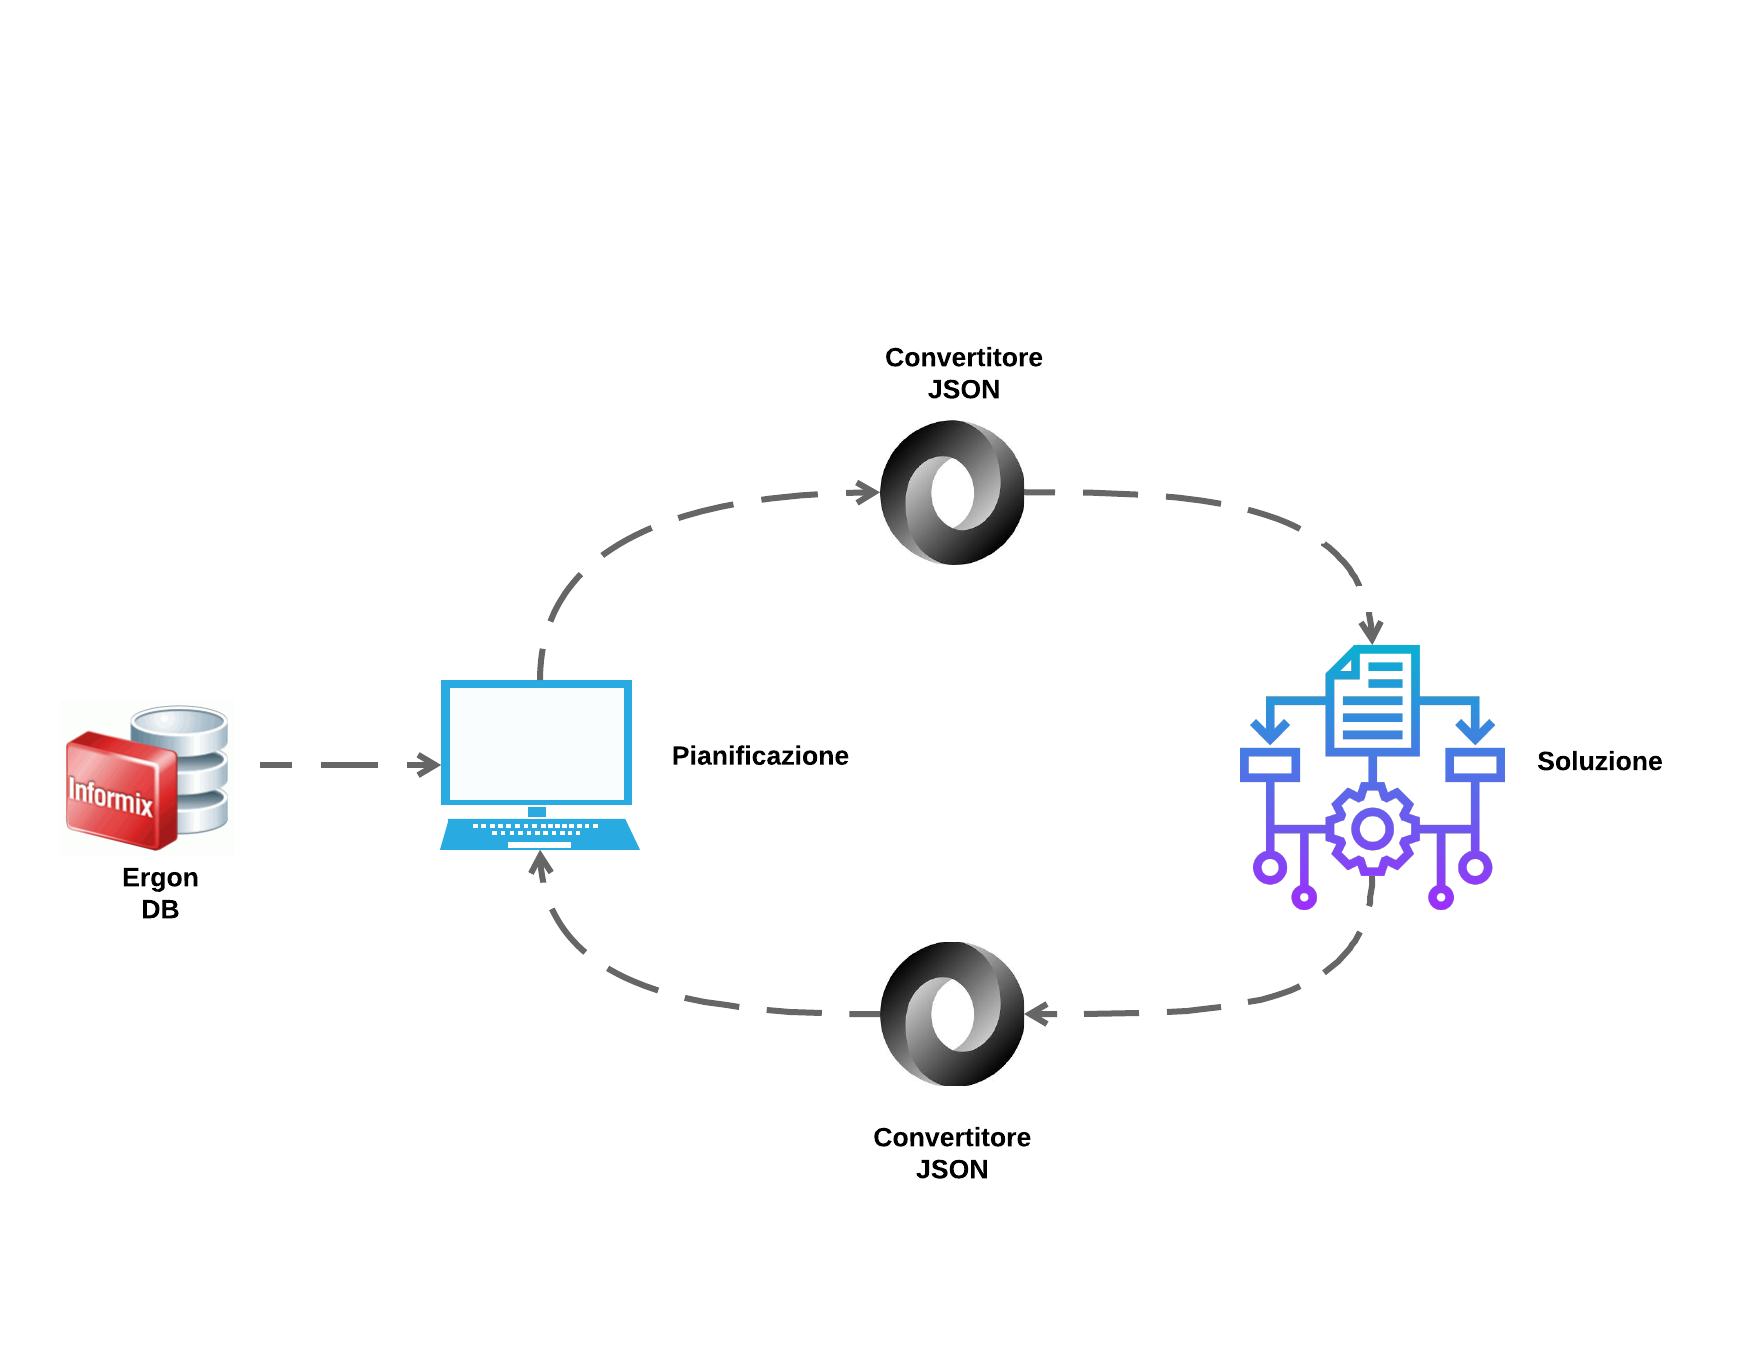
\includegraphics[width=13cm]{immagini/architettura.png}
	\centering
    \caption{Architettura generale}
    \label{4.1}
\end{figure}

\subsection{Algoritmo}

\textbf{Il problema}

Il problema della pianificazione della produzione rientra nella categoria \hyperref[Np-hard]{NP-hard\glo} in quanto è riconducibile al problema del 
\hyperref[Commesso viaggiatore]{commesso viaggiatore\glo} \hyperref[commesso]{\textsuperscript{16}}. 
In aggiunta al problema del commesso viaggiatore si devono considerare
altri vincoli come: 
\begin{itemize}
    \item tempo massimo sul quale si vogliono pianificare gli ordini;
    \item numero di linee sulle quali si possono produrre determinati ordini;
    \item vincoli generali di sequenza che andremo a definire in seguito.
\end{itemize}

Queste caratteristiche avevano portato, nella precedente fase del progetto, a optare per lo sviluppo di algoritmi di soluzione \hyperref[Euristica]{euristici\glo [16]}.
Con la richiesta di estendere tale progetto, il numero di vincoli da soddisfare cresce in proporzione al numero di ordini che si vogliono pianificare.
In particolare vanno tenuti in considerazione i vincoli precedenti più l'aggiunta dei seguenti:

\begin{itemize}
    \item pianificazione dei semilavorati antecedente ai prodotti finiti;
    \item materie prime e semilavorati presenti in quantità sufficienti per la produzione;
    \item verifica della disponibilità di materie prime e semilavorati in base agli ordini fornitori.
\end{itemize}

In conclusione, il problema che il progetto si pone di risolvere, consiste nel trovare una soluzione ammissibile, quanto più vicina all'ottimo,
della pianificazione
in base ai vincoli imposti.\newline

\textbf{La soluzione}

Dovendo appoggiarsi all'algoritmo esistente, non è stato possibile eseguire uno stravolgimento completo del suo funzionamento, anzi si è cercato di inserire le nuove funzionalità
in modo da integrarle il più possibile, senza effettuare modifiche sostanziali, alla struttura del codice esistente.\\ Per fare ciò, si è fatto ampio uso di nuove funzioni e
classi, in modo da garantire un alto grado di modularità del codice aggiunto a quello esistente.
\\ La struttura di partenza sulla quale vengono integrati i nuovi moduli è composta da una fase iniziale
di lettura dei dati dal database. Tali dati vengono convertiti in un file JSON che, per comodità di esecuzione, viene letto nuovamente dallo stesso programma, anche se
l'dea di base sarebbe quella di delegare la sua lettura e successiva elaborazione dei dati ad un sistema centralizzato esterno all'azienda che fornisce i dati stessi.\\
Una volta ottenuti i dati in formato JSON, vengono inseriti nell'algoritmo tramite l'impiego di classi e strutture predisposte. Tali classi vengono utilizzate come parametri
per la prima funzione che si pone come obiettivo quello di fornire una soluzione ammissibile nel minor tempo possibile attraverso un algoritmo \hyperref[Greedy]{Greedy\glo}.\\
Tale algoritmo ha il compito di valutare, in modo sequenziale, i vari ordini che necessitano di essere pianificati, se un ordine soddisfa i vincoli imposti allora verrà inserito nella soluzione iniziale.
Una volta ottenuta la soluzione iniziale, questa viene fornita alla successiva funzione di ottimizzazione, composta da un algoritmo di \hyperref[Tabu Search]{Tabu Search\glo}. Tale algoritmo ha il compito
di eseguire un insieme di mosse specifiche in modo casuale, valutando di volta in volta la bontà della soluzione ottenuta dopo la loro esecuzione. Al termine di un numero prefissato
di iterazioni, o dopo aver soddisfatto i criteri di terminazione, verrà fornita la soluzione "ottimizzata" da visualizzare.\\
Di seguito viene illustrato il funzionamento degli algoritmi adottati, ottenuti dall'integrazione dei precedenti algoritmi.\\

\textbf{Algoritmo Greedy}

L'algoritmo Greedy \hyperref[greedy]{[17]} è il primo passo per ottenere una soluzione ammissibile del problema in questione. Tale algoritmo è sviluppato tenendo in considerazione che non è possibile effettuare dei "passi indietro",
ovvero, una volta inserito un ordine in pianificazione tale ordine rimane fino alla fine dell'esecuzione. I parametri in ingresso di tale algoritmo sono i seguenti:
\begin{itemize}
    \item ordini da pianificare;
    \item materie prime e semilavorati presenti in magazzino;
    \item materie prime e semilavorati presenti in ordini fornitori;
    \item linee di lavorazione con i rispettivi vincoli.
\end{itemize}

L'ordine di funzionamento è quindi il seguente:

\begin{itemize}
    \item prima scelta \hyperref[Euristica]{euristica\glo}, vengono ordinati i prodotti in base alla loro data di spedizione;
    \item il primo ordine in questione viene valutato;
    \item si verifica la presenza di materie prime, e qui abbiamo i seguenti casi:
            \begin{itemize}
                \item le materie prime sono disponibili per produrre l'ordine, inserisco in pianificazione;
                \item le materie prime non sono disponibili per produrre l'ordine, verifico l'arrivo di eventuali materie prime da parte dei fornitori,
                 se ciò avviene inserisco in pianificazione;
                \item non pianifico l'ordine.
            \end{itemize}
    \item si verifica la presenza di semilavorati, e qui abbiamo i seguenti casi:
            \begin{itemize}
                \item i semilavorati sono disponibili per produrre l'ordine, inserisco in pianificazione;
                \item i semilavorati non sono disponibili per produrre l'ordine, provo ad eseguire la pianificazione dei semilavorati mancanti, se ciò avviene
                inserisco in pianificazione;
                \item non pianifico l'ordine.
            \end{itemize}
    \item ogni valutazione effettua un controllo se è possibile inserire l'ordine in base al tempo lavorativo rimanente;
    \item si ripetono le azioni sopracitate fino al termine della valutazione di tutti gli ordini da pianificare.
\end{itemize}

Si ricorda che non è necessario che tutti gli ordini richiesti siano inseriti nella pianificazione, in quanto uno dei precedenti vincoli può non essere soddisfatto e, se tale ordine venisse
inserito nella soluzione, quest'ultima sarebbe non ammissibile perché viola appunto almeno uno dei vincoli imposti. Inoltre, se si esegue un accurato controllo, si può notare che 
il risultato fornito al termine della sua esecuzione, in alcuni casi, ha un ampio margine di miglioramento. L'algoritmo Greedy ha come obiettivo quello di creare una
soluzione iniziale nel modo più rapido possibile, in modo da ottenere una base di partenza per la successiva ottimizzazione eseguita dall'algoritmo Tabu Search.\\


\textbf{Tabu Search}

Una volta ottenuta la prima soluzione ammissibile, fornita dall'algoritmo Greedy, l'esecuzione si sposta sulla sua ottimizzazione tramite la Tabu Search \hyperref[tabu]{[18]}.
Questa particolare tecnica meta-euristica ha lo scopo di fornire una soluzione\hyperref[scheduling]{[20]}, più vicina all'ottimo, tramite l'esecuzione di mosse che perturbano
la soluzione corrente alla ricerca iterativa di soluzioni sempre migliori. L'esecuzione di queste mosse in modo casuale porta ogni volta ad una nuova soluzione ammissibile, tale risultato viene poi confrontato con la soluzione
precedente, se il risultato è migliorativo allora verrà considerato come nuova miglior soluzione e si utilizzerà per la successiva iterazione, altrimenti tale risultato 
verrà semplicemente scartato e si prosegue con l'esecuzione della mossa successiva. Di seguito è presentato l'ordine di funzionamento di tale algoritmo:
\begin{enumerate}
    \item selezione casuale della mossa da eseguire tra le seguenti:
    \begin{itemize}
        \item mossa aggiungi articolo;
        \item mossa sposta articolo;
        \item mossa scambia articoli;
        \item mossa elimina articolo;
        \item mossa sposta sequenza; 
        \item mossa scambia sequenza.  
    \end{itemize}
    \item validazione della mossa scelta, tramite l'utilizzo della \hyperref[Tabu List]{Tabu List\glo} \hyperref[list]{[21]};
    \item esecuzione della mossa scelta;
    \item valutazione della nuova soluzione in rapporto con la soluzione precedente;
    \item viene ripetuta l'esecuzione nell'ordine sopracitato fino al termine del numero massimo di iterazioni, del tempo imposto o del soddisfacimento di uno dei criteri di
    terminazione.\\
\end{enumerate}


\textit{Scelta della mossa}\\
È utile entrare maggiormente nel dettaglio dei punti precedenti per avere un'idea di come si ottiene la soluzione ottimizzata.\\
Al punto uno, la scelta della mossa, viene eseguita in modo casuale. Durante lo stage, la scelta casuale è stata integrata attraverso l'impiego di alcuni metodi di \hyperref[Diversificazione]{diversificazione\glo} o \hyperref[Intensificazione]{intensificazione\glo}. 
In modo da "forzare" la successiva mossa da scegliere,
quindi non rendendola più completamente casuale. Nel caso dell'intensificazione si punta a scegliere l'insieme di mosse che, ad esempio, nelle loro esecuzioni precedenti hanno fornito
risultati migliori e quindi si pensa potranno fornire migliori risultati anche in futuro, in questo modo ci si concentra maggiormente su queste scartando le altre.\\
Al contrario, la diversificazione può decidere di eseguire le mosse che sono state meno eseguite in precedenza così da indirizzare i risultati verso strade mai 
percorse.\\ È proprio quest'ultimo caso che, a seguito di una discussione con il tutor aziendale, è stato inserito nel programma esistente. Il suo funzionamento è semplice ma non banale:
dopo l'esecuzione di metà delle iterazioni concesse alla Tabu Search entra in gioco tale meccanismo, si è deciso di considerare l'esatta metà così da poter ottenere inizialmente una
soluzione meno forzata possibile, da tale momento in poi verrà assegnato un peso percentuale ad ogni mossa che diminuirà ad ogni esecuzione della stessa, aumentando quindi il 
peso delle rimanenti.\\ 
Si è scelto di utilizzare questo metodo per poter garantire comunque un alto grado di casualità, criterio che, nel precedente algoritmo, si è rivelato importante per le prestazioni.\\

\textit{Validazione della mossa scelta}\\
Anche in questo caso è utile approfondire come avviene la validazione di una mossa scelta in modo casuale. In particolare, in alcuni casi, possiamo direttamente scartare
l'esecuzione della mossa perché siamo sicuri che porterà ad una soluzione non migliorativa.\\ Ogni algoritmo di Tabu Search fa affidamento su una relativa 
Tabu List , la quale non è altro che uno storico delle mosse eseguite in precedenza, le quali non dovranno essere rieseguite, almeno nell'immediato futuro.\\
Un criterio importante da tenere presente
è la lunghezza che si sceglie di dare a tale lista, questo perché una lista troppo corta non garantisce che non vengano eseguite mosse utilizzate da poco tempo, mentre, una 
lista troppo lunga tende a creare troppa diversificazione delle soluzioni.\\ Nel progetto di stage alla Tabu List veniva aggiunta anche la mossa opposta a quella eseguita, in modo
da salvare sia la mossa che ha portato ad una nuova soluzione, sia la sua mossa opposta, evitando così di tornare casualmente alla soluzione precedente. 
La validazione di una mossa,
in seguito, deve inoltre sottostare a dei vincoli che appartengono alla realtà sulla quale si basa il nostro applicativo. Ad esempio, se viene considerata la mossa \textit{aggiungi articolo}
ma non abbiamo nessun articolo da aggiungere, tale mossa viene scartata.\\ Con l'aggiunta della pianificazione dei semilavorati, i quali ricordiamo avere le stesse peculiarità
dei prodotti finiti, sono stati aggiunti ulteriori controlli, in quanto non possiamo garantire l'eliminazione tramite la mossa \textit{elimina articolo} di uno di questi senza
eliminare anche l'articolo a cui fanno riferimento.\\ Perciò si è scelto di eseguire l'eliminazione solo sui prodotti finiti. Altri controlli da eseguire riguardano lo spostamento
di articoli o sequenze, nel caso venga selezionato lo spostamento di un semilavorato bisogna accertarsi che non venga inserito in pianificazione successivamente al relativo
prodotto finito. Allo stesso modo è stato necessario aggiungere controlli sulla giacenza e sull'arrivo di merci dai fornitori, questo perché lo spostamento, l'eliminazione e l'aggiunta
di articoli creava una forte oscillazione nei dati riguardanti i materiali da lavorazione e spesso riconduceva ad una soluzione peggiorativa.\\ Come si può intuire, l'aggiunta
di tutti questi vincoli ha minato la capacità di ottenere una soluzione nettamente migliorativa da parte della Tabu Search.\\

\textit{Esecuzione della mossa scelta}\\
Una volta accertati che la mossa sia eseguibile si passa alla sua implementazione.\\ Ogni mossa è correlata ad un insieme di funzioni che hanno il compito di accertarsi che ad
ogni passo della sua esecuzione ci si trovi all'interno di una soluzione ammissibile. È facile riscontrare che, durante l'esecuzione di una di queste mosse, si possa terminare 
in una soluzione non ammissibile, in questo caso viene scartato il nuovo risultato e si torna alla soluzione ammissibile precedente.\\ Nel caso in cui siano soddisfatti tutti
i vincoli imposti al termine dell'esecuzione di una mossa la soluzione ottenuta sarà ammissibile e sarà compito del prossimo passo dell'algoritmo accertarne la bontà.\\

\textit{Valutazione della soluzione}

Una volta ottenuta un nuova soluzione è necessario valutarla per sapere se sia migliorativa o peggiorativa rispetto alla precedente.\\
Il confronto quindi viene eseguito calcolando il punteggio della nuova soluzione il quale è dato dalla seguente funzione:
%\[F(s) = \frac{Pz}{Pz\ped{tot}}*Peso\ped{pz} - \frac{T\ped{linee}}{T\ped{linee-tot}}*Peso\ped{pz}\]

\[\frac{\text{Pezzi pianificati}}{\text{Totale pezzi richiesti}} \times \text{Peso del rapporto pezzi}\]\\

Qui otteniamo il punteggio di maggior spessore, dal quale si sottraggono i seguenti:

\[\frac{\text{Occupazione linee}}{\text{Massima occupazione linee}} \times \text{Peso del rapporto occupazione}\]\\

\[\frac{\text{Tempo totale di pianificazione}}{\text{Massimo tempo a disposizione}} \times \text{Peso del rapporto tempo}\]\\

Una volta ottenuto il relativo punteggio viene eseguito il confronto con la soluzione precedente e si sceglie la soluzione avente il punteggio più alto.\\
Questo non è l'unico metodo con il quale si sceglie la soluzione che riteniamo essere migliore.\\ Vengono impiegati dei criteri di \hyperref[Criteri di aspirazione]{aspirazione\glo} i quali hanno il compito
di valutare anche soluzioni che hanno punteggi inferiori alla precedente ma che potrebbero essere un buon punto di partenza per la valutazione di soluzioni successive.\\
Nel progetto è stato inserito un criterio di aspirazione con il seguente funzionamento: se la nuova soluzione ha un punteggio inferiore alla soluzione precedente, ma il 
numero di pezzi prodotti è superiore, allora se la differenza è inferiore al 2\% la nuova soluzione è considerata migliore. Questo perché lo scopo ultimo della pianificazione
è riuscire a pianificare il maggior numero di ordini possibili.


\subsection{Codifica}

In questa sezione vengono illustrati i vari passi che seguiti durante la fase di codifica del progetto, specificando i punti fondamentali di ognuno.\\

\title{Implementazione controllo giacenze}

Il primo obiettivo che da raggiungere riguardava l'esecuzione della pianificazione in base alle materie prime e semilavorati presenti in magazzino.
Per fare ciò, sono stati eseguiti i passi presentati di seguito:\\ \\
\textbf{Controllo giacenze}
\begin{enumerate}
        \item lettura dal database dei dati riguardanti le giacenze;
        \item utilizzo di una funzione di esplosione distinta per ottenere la \hyperref[Distinta base]{distinta base\glo} dei prodotti finiti; 
        \item scrittura dei dati in un file JSON;
        \item creazione di una classe volta a lavorare sulle giacenze;
        \item creazione di una funzione volta al controllo della presenza di materiali per eseguire la pianificazione;
        \item integrazione di tale funzione con gli algoritmi Greedy e Tabu Search;
        \item rimozione dei materiali necessari a produrre un prodotto finito;
        \item reintegrazione dei materiali in magazzino se uno o più articoli vengono eliminati dalla pianificazione.\\
\end{enumerate}

\textbf{Pianificazione semilavorati} 
\begin{enumerate}
        \item utilizzo di una funzione di esplosione distinta per ottenere la distinta base dei prodotti finiti; 
        \item scrittura dei dati in un file JSON;
        \item riutilizzo della classe \textit{Ordine} per i semilavorati;
        \item ampliamento delle funzionalità della classe \textit{Ordine} per tenere traccia dei semilavorati di ogni prodotto finito;
        \item integrazione della pianificazione dei semilavorati nell'algoritmo Greedy, anticipando la loro produzione rispetto al prodotto finito;
        \item inserimento di controlli ausiliari per impedire spostamenti ed eliminazioni durante l'esecuzione dell'algoritmo di Tabu Search.\\
\end{enumerate}

In \hyperref[pian-semilavorati]{Figura 4.2} è mostrato come si presenta la pianificazione restituita dall'applicativo dopo la pianificazione dei semilavorati.

\begin{figure}[H]
	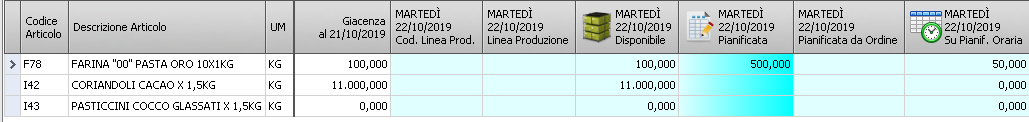
\includegraphics[width=\textwidth]{immagini/sl_planning.png}
	\centering
\end{figure}
\begin{figure}[H]
	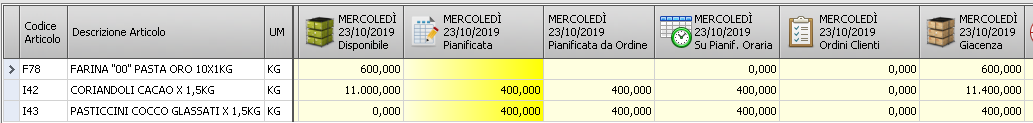
\includegraphics[width=\textwidth]{immagini/sl_planning2.png}
    \centering
    \caption{Pianificazione semilavorati}
    \label{pian-semilavorati}
\end{figure}

Dalla \hyperref[pian-semilavorati]{Figura 4.2} vediamo che \textit{F78} è un semilavorato, di cui abbiamo 100kg in giacenza, richiesto dai prodotti finiti \textit{I42} e \textit{I43}.\\
Sappiamo che i due prodotti finiti in questione richiedono 300kg del semilavorato \textit{F78} ciascuno, e vediamo che il martedì ne sono pianificati esattamente 500kg
per garantire la produzione di \textit{I42} e \textit{I43} il mercoledì.

\newpage

\textbf{Controllo ordini fornitori} 
\begin{enumerate}
        \item lettura dal database i dati riguardanti gli ordini fornitori; 
        \item scrittura dei dati in un file JSON;
        \item creazione di una classe volta a lavorare sugli ordini fornitori;
        \item ampliamento della funzione dedita al controllo delle giacenze;
        \item integrazione di tale funzione con gli algoritmi Greedy e Tabu Search;
        \item inserimento di controlli ausiliari per evitare di ottenere soluzioni non ammissibili durante l'esecuzione di entrambi gli algoritmi.\\
\end{enumerate}

\textbf{Pianificazione ordini da magazzino} 
\begin{enumerate}
        \item lettura di ordini da inserire in pianificazione direttamente dal magazzino;
        \item scrittura dei dati in un file JSON;
        \item riutilizzo della classe \textit{Ordine} per gli ordini da magazzino;
        \item utilizzo di tutti i vincoli precedenti per effettuare la pianificazione.\\
\end{enumerate}

\textbf{Criteri di Diversificazione/Intensificazione}\\ \\

Per ottenere il massimo dall'esecuzione dell'algoritmo di Tabu Search, si è infine scelto di utilizzare una tecnica di diversificazione come spiegato nella sezione precedente \hyperref[criteria]{[22]}.

\newpage

\section{Verifica e validazione}

La fase di verifica si è protratta durante tutta la fase di sviluppo del progetto. Sono state impiegate delle tecniche di analisi statica, in quanto non era previsto un piano di test
da effettuare sui risultati ottenuti.\\ Il non eseguire dei test automatici sui risultati ottenuti deriva anche dal fatto che i dati utilizzati corrispondano
a dei dati reali, per i quali sarebbe stato più complicato codificare un insieme di test automatici. La problematica precedente avrebbe sottratto un considerevole ammontare di tempo allo sviluppo del
codice applicativo. 

\subsection{Analisi statica}

Si è fatto ampio uso dello strumento di debug fornito da Visual Studio 2010 e ho creato una lista di controllo tramite \hyperref[Breakpoint]{breakpoint\glo} in modo da poter
valutare, durante l'esecuzione, lo stato del software ad ogni punto critico. Ciò ha permesso di individuare efficacemente gli errori a livello logico che si sono presentati
durante la varie fasi di sviluppo. Si è proseguito poi con dei controlli a campione della soluzione presentata a video dal programma, 
valutando determinati ordini, in modo da ottenere un riscontro reale della bontà della soluzione stessa. 

\subsection{Analisi dinamica}

Si è fatto uso di più funzioni con il compito di attestare che la soluzione corrente sia ammissibile, in particolare ogni funzione aveva il compito di verificare che
determinati vincoli fossero rispettati. Ad esempio, dopo aver inserito il controllo sulle materie prime e semilavorati, veniva verificato che la rimozione di queste due componenti
combaciasse con quanto risultava presente in magazzino. Sono stati effettuati altri controlli sul tempo di pianificazione rimanente e vincoli di linea imposti dalle relative
aziende. Si sottolinea che queste funzioni vengono richiamate solo in punti ben definiti nel codice, in quanto non sarebbe utile richiamare la stessa funzione di controllo
se i vincoli che attesta non sono stati modificati nella soluzione. Nel caso in cui una di queste funzioni accertasse l'inammissibilità della soluzione corrente veniva 
lanciata un eccezione, la quale riportava il vincolo che non era stato soddisfatto.


\subsection{Validazione}

Al raggiungimento di ogni stato rilevante dell'applicativo veniva eseguito un collaudo. Questo aveva il compito di accertare che i risultati ottenuti fossero in linea con
quanto ci si aspetta dalla pianificazione reale. Per fare ciò si eseguiva l'applicativo con i dati reali di una specifica azienda, dei quali si era giunti ad ottenere
una soluzione relativamente buona. Una volta confrontate le due soluzioni evidenziavo le eventuali discrepanze e passavo ad una verifica accurata di quanto ottenuto.
Seguiva poi una discussione con il tutor interno per accertarsi che tali scostamenti derivassero dalle nuove aggiunte e non fossero errori logici del programma.\\ Una volta 
accertati che la soluzione ottenuta fosse ammissibile e coerente veniva salvata e impiegata nelle successive fasi di validazione e collaudo.

\section{Risultati dei test}

Di seguito vengono riportati i risultati sui test effettuati durante le varie fasi di sviluppo del progetto. Sono presentati in forma grafica così da garantire un'immediata
comprensione.\\ I dati utilizzati per ottenere questi risultati fanno parte degli ordini, delle giacenze di magazzino 
e degli ordini fornitori di uno specifico cliente di Ergon Informatica.\\
Ogni test è stato effettuato sullo stesso ammontare di ordini distribuito in una singola settimana lavorativa, questo per garantire una continuità tra i vari test eseguiti.\\
L'insieme dei dati utilizzati sono i seguenti:
\begin{itemize}
    \item Numero ordini = 273;
    \item Numero semilavorati = 183;
    \item Numero giacenze = 525;
    \item Numero ordini fornitori = 57.
\end{itemize}

Si precisa che non tutti gli ordini devono essere pianificati e che vengono presi in considerazione solo i dati riguardanti la settimana corrente di pianificazione.
Ogni grafico è presentato in due diverse versioni, una tramite grafico a barre per confrontare le diverse misurazioni e una tramite grafico a dispersione per evidenziare
l'andamento della soluzione.
\subsection{Pianificazione prodotti finiti}

In \hyperref[4.3]{Figura 4.3} viene rappresentato l'andamento temporale dell'esecuzione dell'algoritmo Greedy e Tabu Search al variare del numero di iterazione massime consentite.

\begin{figure}[H]
	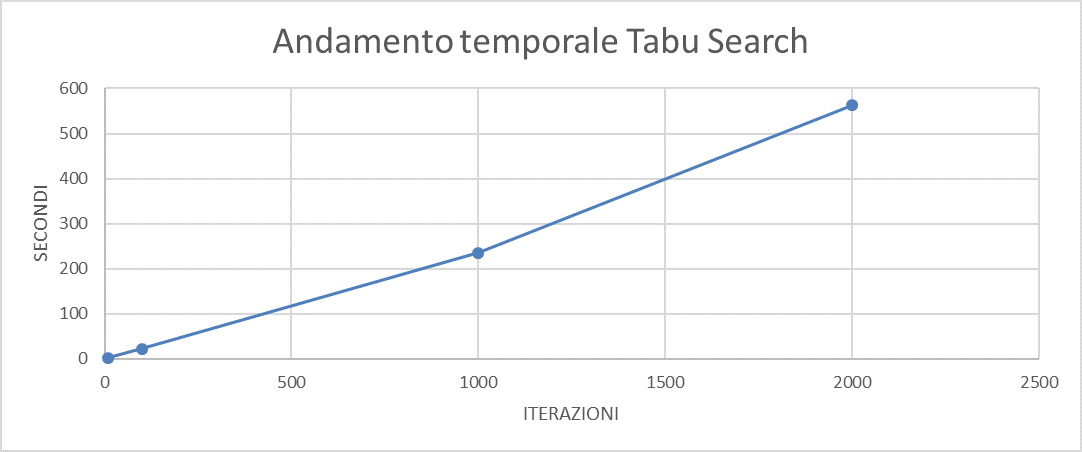
\includegraphics[width=13cm]{immagini/graficoPF2.png}
	\centering
	\caption{Grafico temporale della pianificazione dei prodotti finiti}
    \label{4.3}
\end{figure}

Per quanto riguarda il tempo di esecuzione dell'algoritmo Tabu Search vediamo un aumento in proporzione al variare del numero di iterazioni.
In \hyperref[4.4]{Figura 4.4} viene mostrato il miglioramento in percentuale, rispetto alla soluzione fornita dall'algoritmo Greedy, ottenuto dall'algoritmo di ottimizzazione.

\begin{figure}[H]
	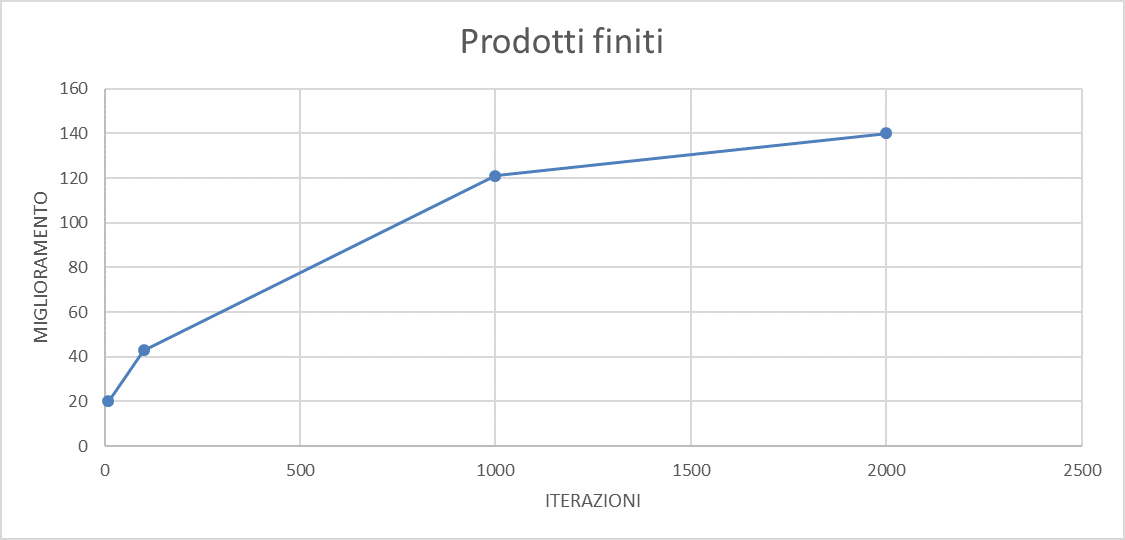
\includegraphics[width=13cm]{immagini/graficoPF3.png}
	\centering
    \caption{Grafico miglioramento percentuale della soluzione della pianificazione dei prodotti finiti}
    \label{4.4}
\end{figure}

Dopo vari test eseguiti posso affermare che, considerando anche il tempo impiegato, il numero di iterazioni ideale si assesti tra le 1000 e 2000 iterazioni.
Superate le 2000 iterazioni il miglioramento assume un andamento asintotico ed evidenzia solo uno spreco di tempo di esecuzione. 

\newpage
\subsection{Pianificazione semilavorati}

In \hyperref[4.5]{Figura 4.5} sono rappresentati i risultati dei test eseguiti dopo il primo importante avanzamento del progetto ovvero la pianificazione dei semilavorati.

\begin{figure}[H]
	\includegraphics[width=13cm]{immagini/graficosl2.png}
	\centering
    \caption{Grafico temporale con aggiunta della pianificazione dei semilavorati}
    \label{4.5}
\end{figure}

La prima cosa da notare è l'aumento del tempo di esecuzione da parte dell'algoritmo Greedy, il quale necessita ora di un elevato numero di controlli aggiuntivi. La funzione
stessa è stata resa \hyperref[Ricorsione]{ricorsiva\glo} in modo da riutilizzare il codice al suo interno per eseguire la pianificazione dei semilavorati. Questo ha permesso anche di creare una
relazione diretta tra il semilavorato e il suo prodotto finito, il tutto tramite una relazione padre figlio creata appositamente nella classe.
In compenso, l'algoritmo di Tabu Search non ha subito un aumento considerevole del tempo di esecuzione ma ha subito un calo drastico nella capacità di ottimizzazione della
soluzione.

\begin{figure}[H]
	\includegraphics[width=13cm]{immagini/graficosl3.png}
	\centering
    \caption{Grafico miglioramento percentuale della soluzione della pianificazione dei semilavorati}
    \label{4.6}
\end{figure}

Come possiamo notare in \hyperref[4.6]{Figura 4.6}, al termine delle 2000 iterazioni, il fattore di miglioramento si aggira attorno 19\%. Questo è dovuto al fatto che l'algoritmo
si trova di fronte a un elevato numero di controlli ausiliari prima di poter eseguire una mossa. Si prenda ad esempio la mossa di eliminazione, non può essere effettuata su un semilavorato
per questioni logico/reali in quanto non sarebbe più possibile pianificare il suo prodotto finito relativo. Allo stesso modo non è possibile spostare la pianificazione di un
semilavorato successivamente al suo prodotto finito e viceversa non è possibile pianificare il prodotto finito prima dei suoi semilavorati. Ciò è la causa della perdita di
capacità di ottimizzare la soluzione ottenuta dall'algoritmo Greedy.

\newpage
\subsection{Controllo ordini fornitori}

In aggiunta alla pianificazione dei semilavorati, è stato aggiunto il controllo sull'arrivo di materiale da parte dei fornitori.\\Ciò permette di non scartare a priori la possibilità
di pianificare alcuni ordini che, a causa dell'assenza di materiali, non verrebbero considerati. In questo modo, vengono considerati pianificabili tutti gli ordini per i quali
è presente almeno un ordine fornitore che soddisfa la quantità di materiali necessari. 

\begin{figure}[H]
	\includegraphics[width=13cm]{immagini/graficofo2.png}
	\centering
    \caption{Grafico temporale con aggiunta della pianificazione degli ordini fornitori}
    \label{4.7}
\end{figure}

Come si può notare in \hyperref[4.7]{Figura 4.7} la Tabu Search, anche in questo caso, impiega più tempo al variare del numero di iterazioni, ma rimanendo comunque entro limiti accettabili.

\begin{figure}[H]
	\includegraphics[width=13cm]{immagini/graficofo3.png}
	\centering
    \caption{Grafico miglioramento percentuale della soluzione della pianificazione degli ordini fornitori}
    \label{4.8}
\end{figure}

Dalla \hyperref[4.8]{Figura 4.8} si evince la netta incapacità della Tabu Search di ottenere una soluzione migliore partendo dalla soluzione fornita dall'algoritmo Greedy.\\
Questo avviene perché, in questo caso particolare, molti ordini sarebbero pianificabili per quanto riguarda i materiali a disposizione (cosa non realizzabile per le fasi
precedenti) e questo va a diminuire nettamente il risultato del rapporto pesato \[\frac{\text{Pezzi pianificati}}{\text{Totale pezzi richiesti}} \times \text{Peso del rapporto pezzi}\]\\
dove in \textit{Totale pezzi richiesti} vengono considerati tutti gli ordini producibili.\\ Inoltre, avendo un grandissimo numero di ordini producibili, le mosse eseguite 
dalla Tabu Search non fanno altro che sostituire ordini con altri ordini quindi non può ottenere un miglioramento significativo.

\newpage
\subsection{Criteri di diversificazione}

L'implementazione della tecnica di diversificazione ha portato ai risultai presenti in figura 4.9, dove la linea blu rappresenta la soluzione ottenuta senza i criteri di diversificazione
mentre, la linea rossa rappresenta la soluzione con l'applicazione dei criteri di diversificazione. I dati su cui sono stati eseguiti i seguenti test sono differenti rispetto ai
precedenti, questo perché, verso la fine dello stage, i dati forniti dall'azienda sono cambiati. Inoltre non era necessario valutare direttamente i dati precedenti ma ottenere
una stima del miglioramento basata sullo stesso set di ordini.

\begin{figure}[H]
	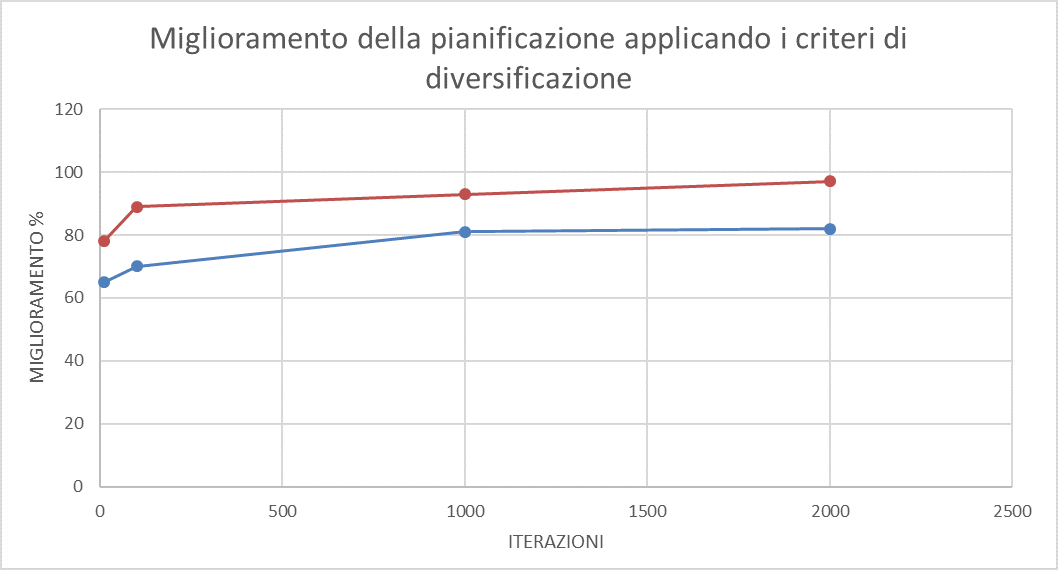
\includegraphics[width=13cm]{immagini/diversificazione.png}
	\centering
    \caption{Grafico miglioramento percentuale della soluzione della pianificazione con l'applicazione di criteri di diversificazione}
    \label{4.9}
\end{figure}

Come possiamo notare dalla \hyperref[4.9]{Figura 4.9}, vi è un miglioramento del 20\% circa della soluzione in ogni stato di esecuzione.\\
Questo evidenzia l'efficacia dei criteri di diversificazione utilizzati.
Inoltre, esaminando le soluzioni fornite pre e post inserimento dei criteri, si può notare che questi ultimi sono più efficaci se è richiesta la pianificazione di un insieme
di ordini aventi un elevato numero di pezzi, trascurando la pianificazione di molti ordini aventi un quantitativo di pezzi inferiore alla media.\\
Tali dati verranno presi in considerazione da Ergon Spa per decidere, in base alle esigenze dei clienti, quale delle due politiche di pianificazione adottare.
             % Concept Preview
% !TEX encoding = UTF-8
% !TEX TS-program = pdflatex
% !TEX root = ../tesi.tex

%**************************************************************
\chapter{Conclusioni}
\label{cap:conclusioni}
%**************************************************************
\section{Consuntivo delle tempistiche}
\label{tempistiche}
La pianificazione oraria ha subito alcuni cambiamenti durante lo stage. Questo perché mi è stato chiesto di dare maggiore priorità ad alcuni elementi ritenuti 
più importanti per l'azienda rispetto ad altri aspetti secondari che potevano essere colmati in altri modi. In particolare la parte di stesura di manuale utente e sviluppatore,
considerata opzionale, è stata tralasciata per dare maggior peso alla parte di test e validazione del prodotto. Inoltre si è scelto, assieme al tutor interno, di utilizzare
come appoggio i commenti a supporto del codice piuttosto che i manuali sopracitati. Anche la fase di stesura dell'analisi dei requisiti ha subito una variazione oraria, in quanto
l'aggiunta dei casi d'uso da me proposti ha ricevuto riscontri positivi ed è proseguita senza intoppi fin da subito.\\ Un lieve aumento lo si nota sulla fase di studio delle
tecnologie utilizzate, in quanto dovevo familiarizzare con strumenti che non avevo mai utilizzato, quali DevExpress e vb.NET, la loro padronanza ha richiesto più del dovuto.\\
Infine, come anticipato, la fase di test e validazione ha subito un aumento in quanto, l'accertamento della bontà della soluzione richiedeva un considerevole ammontare di tempo
sia da parte mia che da parte del tutor interno. Questo tempo ha inoltre incluso la fase di controllo statica del codice durante la stesura delle nuove unità e controlli dinamici
durante l'esecuzione dell'applicativo.
La \hyperref[effettive]{Tabella 5.1} presenta il consuntivo delle ore effettive in relazione alle ore preventivate, a seguito della loro ripianificazione.
Lo sviluppo delle varie componenti non aveva previsto un monte ore per ogni singola attività, vieni indicato quindi con la sigla NP (Non preventivato) le ore non preventivate e 
inserito solo il totale previsto con eventuali variazioni.
\newpage


\renewcommand{\arraystretch}{1.5}
\rowcolors{2}{dispari}{pari}
\arrayrulecolor{white}
\begin{longtable}{ >{\centering}p{0.16\textwidth} >{}p{0.60\textwidth}
    >{\raggedright}p{0.15\textwidth} >{\centering}p{0.14\textwidth}}
	\caption{Ore effettive}
	\label{effettive}
\\
\rowcolorhead 
\textbf{\color{white}Ore preventivate} 
& \textbf{\color{white}Descrizione} 
& \centering\textbf{\color{white}Ore effettive}
 

\endhead	

40	&	Analisi del modulo software esistente, funzionalità da realizzare e documentazione disponibile dell’algoritmo esistente	&	\centering 40	\tabularnewline
4	&	Analisi dei requisiti e stesura della relativa documentazione	&	\centering 4	\tabularnewline
20	&	Studio delle tecnologie aziendali necessarie allo sviluppo del modulo 	&	\centering 20	\tabularnewline
40	&	Studio di algoritmi e tecniche di Ricerca Operativa e Ottimizzazione Combinatoria	&	\centering 40 	\tabularnewline
NP	&	Sviluppo procedura di gestione degli ordini fornitori  & \centering 29 	\tabularnewline
NP	&	Sviluppo procedura di gestione delle giacenze di magazzino  & \centering 15 	\tabularnewline
NP	&	Sviluppo procedura di gestione dei semilavorati pianificati  & \centering 30 	\tabularnewline
NP	&	Integrazione dei vincoli del problema di ottimizzazione con i nuovi parametri  & \centering 24 	\tabularnewline
NP	&	Algoritmo Greedy: sviluppo di nuove strategie di scelta del passo successivo adottato dall’algoritmo nella costruzione della soluzione del problema  & \centering 12 	\tabularnewline
NP	&	Integrazione della Tabu Search con nuovi meccanismi: criteri di aspirazione e arresto, variazione dei meccanismi di esplorazione del vicinato e adozione di tecniche di intensificazione e diversificazione  & \centering 22 	\tabularnewline
	TOTALE:132	&		&	\centering 132 	\tabularnewline
	60	&	Validazione e test	&	\centering 80(+20) 	\tabularnewline
24	&	Stesura della documentazione del prodotto sviluppato	&	\centering 4(-20) 	\tabularnewline
\end{longtable}

\newpage
\section{Consuntivo dell'analisi dei rischi}

Si sono verificati due dei tre casi preventivati nella fase di analisi dei rischi, come evidenziato in \hyperref[rischi2]{Tabella 5.2}.\\ Il primo riguarda il rischio \textit{RT1-Inesperienza tecnologica} con il quale mi sono
scontrato nelle prime fasi del progetto. Il secondo riguarda \textit{RT2-Scelte implementative} il quale ha richiesto maggior tempo di verifica durante la codifica.


\renewcommand{\arraystretch}{1.5}
\rowcolors{2}{dispari}{pari}
\arrayrulecolor{white}
\begin{longtable}{ >{\centering}p{0.45\textwidth} >{}p{0.45\textwidth}
    >{\raggedright}p{0.15\textwidth} >{\centering}p{0.14\textwidth}}
	\caption{Consuntivo dell'analisi dei rischi}
	\label{rischi2}
\\
\rowcolorhead 
\textbf{\color{white}Descrizione} 
& \textbf{\color{white}Soluzione} 
 

\endhead	

Le nuove tecnologie da utilizzare si sono verificate più complicate del previsto, causato anche dal fatto di dover ampliare un progetto già esistente
con diverse funzionalità avanzate già implementate &	Ho fatto uso della documentazione a supporto dell'applicativo e dell'aiuto del tutor interno che mi dava
indicazioni ad ogni passo di esecuzione dell'algoritmo		\tabularnewline
Le varie scelte implementative spesso conducevano a strade senza uscita, dalle quali era necessario ricominciare con una nuova progettazione del codice	&
Tramite l'aiuto del tutor interno e delle conoscenze ormai acquisite sono sempre riuscito a trovare tecniche alternative per portare al termine il progetto	\tabularnewline

\end{longtable}

\newpage
\section{Soddisfacimento dei requisiti e raggiungimento degli obiettivi}

Tutti i requisiti obbligatori sono stati soddisfatti, i quali formavano le fondamenta del progetto di stage ed erano considerati di fondamentale importanza per l'azienda.
Si è raggiunta la totalità dei requisiti desiderabili, i quali davano lustro alle funzionalità dell'applicativo e ne accrescevano l'insieme di funzionalità. I due requisiti
facoltativi non soddisfatti riguardano la stesura dei manuali, convertita in aggiunta di commenti durante la codifica.\\ Viene presentato in \hyperref[soddisfatti]{Tabella 5.3}
il riepilogo dei requisiti soddisfatti.


\renewcommand{\arraystretch}{1.5}
\rowcolors{2}{dispari}{pari}
\arrayrulecolor{white}
\begin{longtable}{ 
		>{\centering}p{0.17\textwidth} 
		>{\raggedright}p{0.28\textwidth}
		>{\raggedright}p{0.29\textwidth} 
		>{\centering}p{0.15\textwidth}
	}
	
	\caption{Requisiti soddisfatti}
	\label{soddisfatti}
	\\
	\rowcolorhead
	\colorhead\textbf{Stato} & \centering\colorhead\textbf{Obbligatori} & 
	\centering\colorhead\textbf{Desiderabili} & 
	\colorhead\textbf{Facoltativi} 
	\tabularnewline
	\endfirsthead
	\rowcolor{white}\caption[]{(continua)}\\
	\rowcolorhead
	\colorhead\textbf{Stato} & \centering\colorhead\textbf{Obbligatori} & 
	\centering\colorhead\textbf{Desiderabili} & 
	\colorhead\textbf{Facoltativi} 
	\tabularnewline
	\endhead
	
	%RO1---------------------------------------------------------
	\rowcolordark  Soddisfatti & 
	\centering 24 &
	\centering 5 &
	\centering 0	
	\tabularnewline
	
	%RO2---------------------------------------------------------
	\rowcolorlight Non soddisfatti & 
	\centering \\0 &
	\centering \\0 &
	\centering \\2	
	\tabularnewline

	
\end{longtable}


Per quanto riguarda gli obiettivi opzionali ne è stato scartato uno in seguito ad un colloquio con il tutor aziendale, secondo il quale non valeva la pena di sovraccaricare il programma con dei
dati ridondati per eseguire una ripianificazione. Si è scelto quindi di pianificare partendo da zero con i nuovi dati. In \hyperref[raggiunti]{Figura 5.1} sono riportati in grafico i requisiti e il loro
Soddisfacimento.\\ Gli altri obiettivi sono stati ampiamente raggiunti durante le rispettive fasi dello sviluppo dell'applicativo.

\begin{figure}[H]
	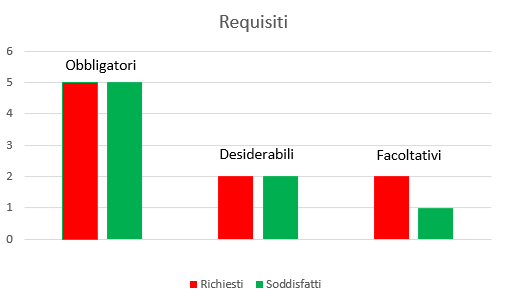
\includegraphics[width=13cm]{immagini/requisiti.png}
	\centering
	\caption{Obiettivi raggiunti}
	\label{raggiunti}
\end{figure}


\section{Conoscenze acquisite}

Durante il percorso di stage ho acquisito nuove conoscenze sia in ambito tecnico che di sviluppo sottostando ad esigenze reali. 

\subsection{Vb.NET, DevExpress e Informix}

Sono le tecnologie che più ho utilizzato durante lo svolgimento dello stage, e mi sono servite durante tutto l'arco di codifica e testing.\\
Essendo la prima volta che mi interfacciavo con queste tecnologie ho riscontrato alcuni problemi in partenza, dovuti appunto all'inesperienza e al fatto che il mio 
progetto si integrava ad uno esistente. La base teorica comunque è riconducibile a qualsiasi altro linguaggio di programmazione visto anche in ambito universitario
per quanto riguarda Vb.NET. \\Per quanto riguarda Informix si sono rese sufficienti le conoscenze teoriche e pratiche conseguite durante il percorso di studi, si è resa
necessario qualche intervento da parte del tutor aziendale in casi particolari di formattazione delle tabelle che andavo ad utilizzare.\\
DevExpress ha avuto un ruolo marginale rispetto ai precedenti ma è comunque servito ad interpretare correttamente le funzionalità dell'interfaccia grafica sulla quale dovevo
apportare le modifiche richieste. Al termine dello stage posso affermare che ho acquisito la piena padronanza di queste tecnologie non solo a livello superficiale ma anche
andando più in profondità, altre conoscenze derivano dal fatto di prolungare il loro utilizzo in futuro.\\

\subsection{Metodo di lavoro}

È la prima volta che mi pongo dinanzi ad un progetto di tali dimensioni, ciò mi ha permesso di imparare a gestire le varie scadenze e consegne entro dei limiti
imposti da un vero e proprio mondo del lavoro. \\Inizialmente ho leggermente sottovalutato le ore di studio del problema esistente, non per negligenza ma perché non mi è parso
chiaro sin da subito l'entità del problema che dovevo affrontare, fino a quando non ho effettivamente iniziato a lavorarci.\\ Ciò ha inizialmente rallentato la fase di sviluppo
in quanto dovevo porre frequenti domande al tutor anche per aiutarmi ad entrare nell'ottica della pianificazione eseguita sui generi alimentari di cui tratta l'azienda.\\ Ciò mi
ha concesso di capire quanto sia importante chiarire ogni dubbio prima di iniziare a lavorare sulla soluzione del problema, così da non causare un effetto cascata in seguito.
Nelle fasi successive, grazie a tale esperienza, non ho avuto problemi al di fuori di questioni legate a vincoli reali di pianificazione ed è stato possibile proseguire senza
rallentamenti.

\subsection{Scadenze}

Anche in questo caso ho dovuto riadattare il mio regime di lavoro in base alle scadenze imposte.\\ Avendo già avuto a che fare con problemi di \hyperref[Scheduling]{scheduling\glo} del lavoro,
mi sono affidato ad un calendario che ho compilato dal primo giorno di stage, nel quale inserivo i vari obiettivi da raggiungere settimanalmente e giornalmente. Con questo
sono riuscito a garantire un ottimo flusso di esecuzione delle operazioni da portare al termine in modo lineare ed efficacie. Nel caso di problematiche esterne ho valutato dei
possibili tempi di stallo nel \hyperref[Planning]{planning\glo} così da avere un margine di scarto in ogni settimana lavorativa.

\section{Università e mondo del lavoro}

Ho sempre avuto la tendenza a valutare il mondo scolastico completamente separato dal mondo del lavoro. Questo perché alcune conoscenze tendono a fermarsi al livello teorico
senza però scendere nel dettaglio e quindi mancanti della parte pratica. Al contrario, nel mondo del lavoro ho sempre pensato che sia la pratica a far da padrone e che quindi
risultasse sì utile il grado di preparazione teorica, ma che non avesse la stessa rilevanza in termini di capacità richieste ad un qualsiasi lavoratore. Dopo questo stage posso
invece affermare che il grado di conoscenza teorico è di gran lunga superiore al grado di conoscenza pratico ed è un elemento fondamentale che un qualsiasi buon programmatore 
deve avere.\\ Durante il progetto ho dovuto spaziare tra diversi campi che vanno dall'Ingegneria del Software alla Ricerca Operativa, passando per altre decine di conoscenze
che se non avessi frequentato l'Università non avrei padroneggiato. Inoltre ho valutato importantissima la capacità di saper imparare nuovi concetti e acquisire informazioni,
grazie al metodo di studio affinato durante il percorso di studi, la quale supera di gran lunga la capacità di saper semplicemente utilizzare un qualsiasi strumento
di sviluppo o simili.\\ In sostanza sono fermamente convinto che anche un percorso di studi triennale fornisca le competenze necessarie e sufficienti per approcciarsi in modo
corretto al mondo del lavoro.

\subsection{Valutazione personale}

L'intero progetto di stage è stato svolto sotto la supervisione del tutor aziendale che però non ha partecipato attivamente allo sviluppo del progetto, anzi ha cercato di 
lasciarmi quanto più spazio possibile cosicché possa trovare da solo una soluzione ai problemi che, molto probabilmente, dovrò riaffrontare in futuro. Ovviamente era sempre
disponibile in caso di problematiche che andassero al di la della mia comprensione in materia di politiche aziendali e anche nel caso in cui dovessi affrontare dei problemi
implementativi di spessore.\\ Il fatto di doversi gestire con le tempistiche e le varie scadenze ha accresciuto molto la mia competenza di giudizio sulle mie reali capacità.
Inoltre il rapporto coi colleghi mi ha aiutato ad entrare, soprattutto mentalmente, nell'ottica lavorativa condivisa in azienda e anche questo mi ha permesso di crescere
a livello personale.\\ In conclusione ritengo il periodo di stage un fattore di crescita personale di fondamentale importanza per uno studente universitario. Ti permette di capire
se il tuo percorso di studi è stato utile e se effettivamente è il lavoro che intendi fare una volta concluso il proprio percorso.\\ Lo ritengo fondamentale in un corso di studi
come il nostro e sono d'accordo che sia obbligatorio per conseguire il titolo di studio.             % Product Prototype
% !TEX encoding = UTF-8
% !TEX TS-program = pdflatex
% !TEX root = ../tesi.tex

%**************************************************************
\chapter{Verifica e validazione}
\label{cap:verifica-validazione}
%**************************************************************             % Product Design Freeze e SOP
% !TEX encoding = UTF-8
% !TEX TS-program = pdflatex
% !TEX root = ../tesi.tex

%**************************************************************
\chapter{Conclusioni}
\label{cap:conclusioni}
%**************************************************************

%**************************************************************
\section{Consuntivo finale}

%**************************************************************
\section{Raggiungimento degli obiettivi}

%**************************************************************
\section{Conoscenze acquisite}

%**************************************************************
\section{Valutazione personale}
             % Conclusioni
\appendix                               
% !TEX encoding = UTF-8
% !TEX TS-program = pdflatex
% !TEX root = ../tesi.tex

%**************************************************************
\chapter{Appendice A}
%**************************************************************

\epigraph{Citazione}{Autore della citazione}



             % Appendice A

%**************************************************************
% Materiale finale
%**************************************************************
\backmatter
\printglossaries
% !TEX encoding = UTF-8
% !TEX TS-program = pdflatex
% !TEX root = ../tesi.tex

%**************************************************************
% Bibliografia
%**************************************************************

\chapter{Riferimenti bibliografici e sitografici}

\begin{enumerate}[label={[\arabic*]}]
    \item \label{sec:ergon} Azienda Ergon Informatica URL: \url{http://www.ergon.it/};
    
    \item \label{sec:ergon2} Azienda e StageIT URL: \url{http://www.ergon.it/index.php?id=new&ine=13};
    
    \item \label{analisi-requisiti} Analisi dei Requisiti: documento interno di Ergon Informatica;
    
    \item \label{uml} Dan Pilone \textit{Uml in a nutshell} 2nd ed. 2005;
    
    \item \label{vbnet} Pagina iniziale Microsoft Visual Basic .NET URL: \url{https://docs.microsoft.com/it-it/dotnet/visual-basic/}
    
    \item \label{vb-logo} Logo Vb.Net URL: \url{https://ingenieriavb.files.wordpress.com/2011/07/visualbasic-net1.png}
    
    \item \label{vs} Pagina iniziale Microsoft Visual studio 2010 URL: \url{https://visualstudio.microsoft.com/it/vs/}

    \item \label{vs-logo} Logo Visual Studio 2010 URL: \url{https://it.wikipedia.org/wiki/Visual_Basic_.NET#/media/File:Visual_basic_2010.png}
    
    \item \label{devexpress} Pagina iniziale DevExpress URL: \url{https://www.devexpress.com/}
    
    \item \label{devlogo} Logo DevExpress URL: \url{http://allvectorlogo.com/devexpress-logo/}
    
    \item \label{json} Pagina iniziale JSON URL: \url{https://www.json.org/json-it.html}
    
    \item \label{jlogo} Logo JSON URL: \url{https://en.wikipedia.org/wiki/JSON#/media/File:JSON_vector_logo.svg}
    
    \item \label{informix} Pagina iniziale Informix URL: \url{https://www.ibm.com/it-it/products/informix}
    
    \item \label{ilogo} Logo Informix URL: \url{https://snbchf.com/2016/04/f-vidocq/informix-logo-png/}
    
    \item \label{slide} Dispense del corso Metodi e Modelli per l'ottimizzazione combinatoria, Luigi De Giovanni URL:
     \url{http://www.math.unipd.it/~luigi/courses/metmodoc/metmodoc.html}

     \item \label{slide0} Dispense del corso di Ricerca Operativa, Luigi De Giovanni URL:
     \url{https://www.math.unipd.it/~luigi/courses/ricop/ricop.html}
    
    \item \label{tabu} Tabu Search for the job-shop scheduling problem with multi-purpose machines,
    Johann Hurink, Bernd Jurisch, and Monika Thole URL: \url{https://core.ac.uk/
    download/pdf/11470194.pdf}

    \item \label{scheduling} The Complexity of Flowshop and Jobshop Scheduling, M. R. Garey, D. S. Johnson,
    Ravi Sethi URL: \url{https://arizona.pure.elsevier.com/en/publications/complexity-of-flowshop-and-jobshop-scheduling}

    \item \label{list} Tabu Search, Fred Glover e Manuel Laguna nel libro di Colin R. Reeves URL:  
    \url{http://leeds-faculty.colorado.edu/glover/222%20-%20Tabu%20Search%20Chapter%20in%201993%20Reeves%20Book.pdf}

    \item \label{criteria} Developing Tabu Search with intensification and diversification for the seriation problem URL: 
    \url{https://ieeexplore.ieee.org/document/8387110}

    \item \label{alert} Descrizione delle funzionalità dell'applicativo: documento interno di Ergon Informatica;
    
    \item \label{breakpoint} Definizione di breakpoint URL: \url{https://docs.microsoft.com/it-it/visualstudio/debugger/using-breakpoints?view=vs-2019}

    \item \label{client/server} Definizione di sistema client/server URL: \url{https://it.wikipedia.org/wiki/Sistema_client/server}

    \item \label{datacenter} Definizione di data center URL: \url{https://www.zerounoweb.it/techtarget/searchdatacenter/guida-al-data-center-cos-e-come-funziona-classificazione-e-vantaggi/}
    
    \item \label{dbms} Definizione di DBMS URL: \url{https://it.wikipedia.org/wiki/Database_management_system}
    
    \item \label{debug} Definizione di Debug URL: \url{https://it.wikipedia.org/wiki/Debugging}
    
    \item \label{distinta-base} Definizione di distinta base URL: \url{https://www.logisticaefficiente.it/wiki-logistica/supply-chain/distinta-base.html}
    
    \item \label{estensione} Definizione di estensione URL: \url{https://simple.wikipedia.org/wiki/Software_extension}

    \item \label{ide} Definizione di IDE URL: \url{https://it.wikipedia.org/wiki/Integrated_development_environment}
    
    \item \label{log} Definizione di Log URL: \url{https://techterms.com/definition/logfile}

    \item \label{multithread} Definizione di Multithreading URL: \url{https://www.geeksforgeeks.org/multithreading-in-operating-system/}
    
    \item \label{planning} Definizione di planning URL: \url{https://en.wikipedia.org/wiki/Planning}
    
    \item \label{ricorsione} Definizione di ricorsione URL: \url{https://it.wikipedia.org/wiki/Algoritmo_ricorsivo}
    
    \item \label{scheduling2} Project management. Pianificazione, scheduling e controllo dei progetti, Harold Kerzner URL: \url{https://www.amazon.it/management-Pianificazione-scheduling-controllo-progetti/dp/8820334267}
    
    \item \label{UI} Definizione di UI URL: \url{https://searchapparchitecture.techtarget.com/definition/user-interface-UI}
\end{enumerate}
\end{document}
